\documentclass[text01.tex]{subfiles}
\begin{document}
%
% section 1.4
%
\section{HTMLで自己紹介のホームページをつくろう}

みなさんがブラウザを使って見てきたホームページは、HTML(エイチ　ティー　エム　エル)という言語で書かれています。
ブラウザがHTMLを\ruby{理解}{りかい}して、ホームページとして\ruby{表示}{ひょうじ}してくれています。
HTMLはテキストエディタで\ruby{編集}{へんしゅう}することができますので、その決まりさえ覚えれば、ホームページはかんたんに作ることができます。
この章では、作り方を学び、自分の\ruby{自己}{じこ}\ruby{紹介}{しょうかい}のホームページを作ります。

\bigskip

\begin{figure}[hb]
  \centering
  \begin{minipage}{15.801cm}
    {\upshape
      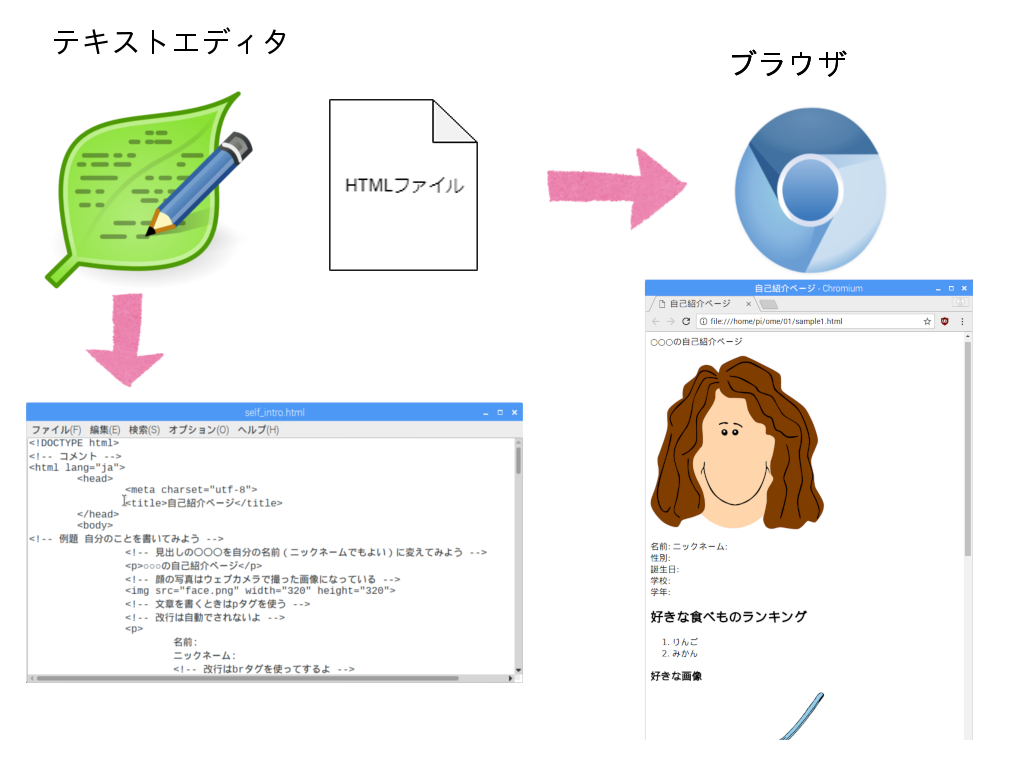
\includegraphics[width=\linewidth]{../../asset/image/textbook-img140.png}
      \caption{ホームページ作成全体図}
    }
  \end{minipage}
\end{figure}
\clearpage


%
% subsection 1.4.1
%
\subsection{教材を\ruby{準備}{じゅんび}しよう}

ホームページの作り方を学ぶための教材は、\texttt{/usr/local/share/ome}というフォルダに置いてあります。
これを、じぶんのフォルダにコピーしましょう。

\textbf{手順}
\vspace{0.5cm}

  % \bigskip

  % \centering
  % \begin{minipage}{\textwidth}
    \begin{minipage}{0.45\linewidth}
      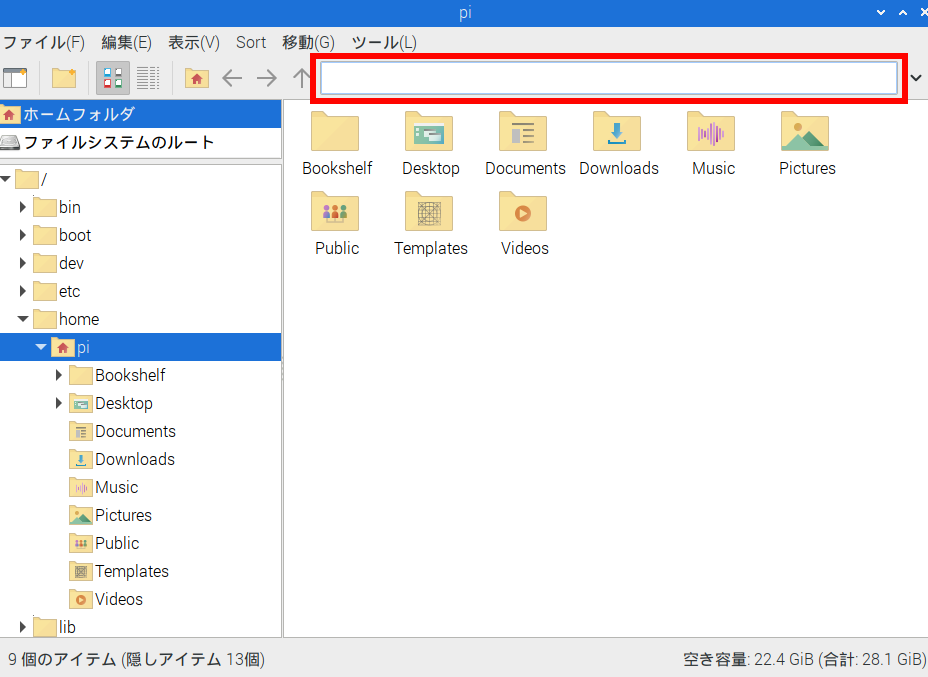
\includegraphics[height=5cm]{../../asset/image/textbook-img1010.png}\\
      \textcircled{\scriptsize{1}} %
      赤い\ruby{枠}{わく}で囲ったところをクリックして、\texttt{/usr/local/share/ome}と入力して、
      エンターキーを\ruby{押}{お}しましょう
    \end{minipage}
    \hfill
    \vspace{20pt}
    \begin{minipage}{0.45\linewidth}
      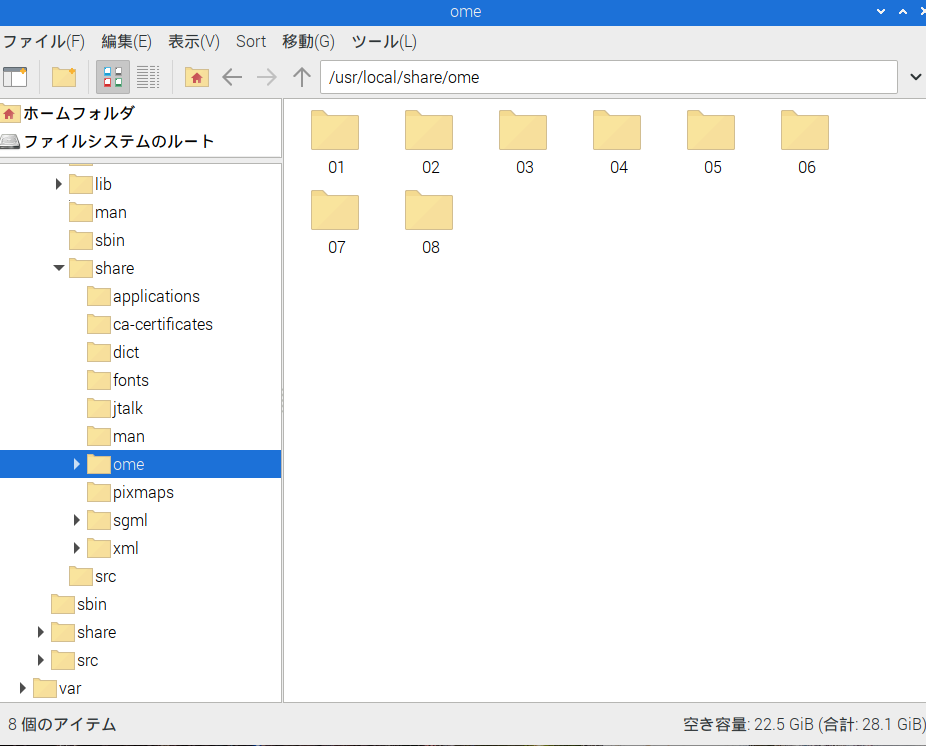
\includegraphics[height=5cm]{../../asset/image/textbook-img1011.png}\\
      \textcircled{\scriptsize{2}} %
      「01」から「08」までのフォルダが\ruby{表示}{ひょうじ}されていることを\ruby{確認}{かくにん}しましょう
    \end{minipage}
    \begin{minipage}{0.45\linewidth}
      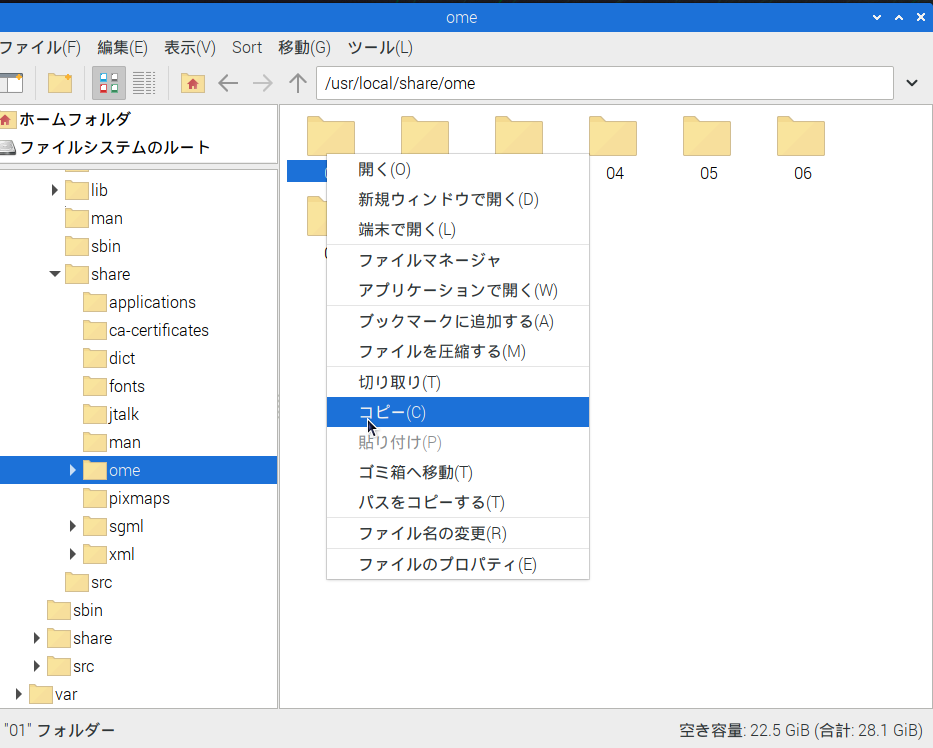
\includegraphics[height=5cm]{../../asset/image/textbook-img1012.png}\\
      \textcircled{\scriptsize{3}} %
      3 「01」フォルダの上で右クリックし、「コピー」しましょう
    \end{minipage}
    \hfill
    \vspace{20pt}
    \begin{minipage}{0.45\linewidth}
      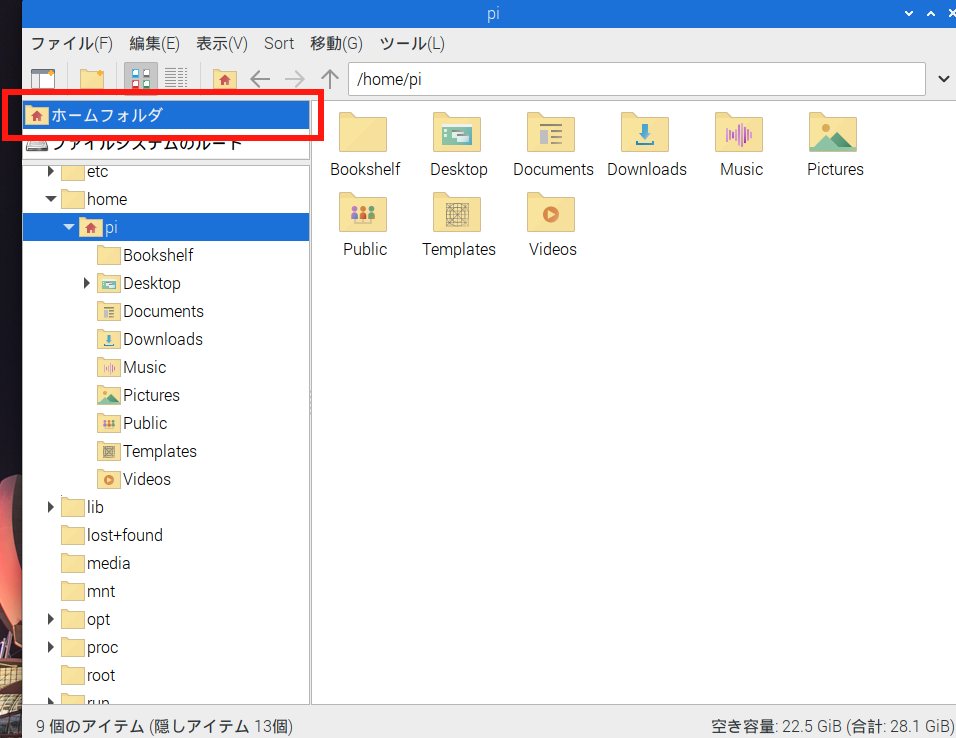
\includegraphics[height=5cm]{../../asset/image/textbook-img1013.png}\\
      \textcircled{\scriptsize{4}} %
      赤い\ruby{枠}{わく}で囲った「ホームフォルダ」をクリックして、自分のフォルダに\ruby{移動}{いどう}しましょう
    \end{minipage}
    \begin{minipage}{0.45\linewidth}
      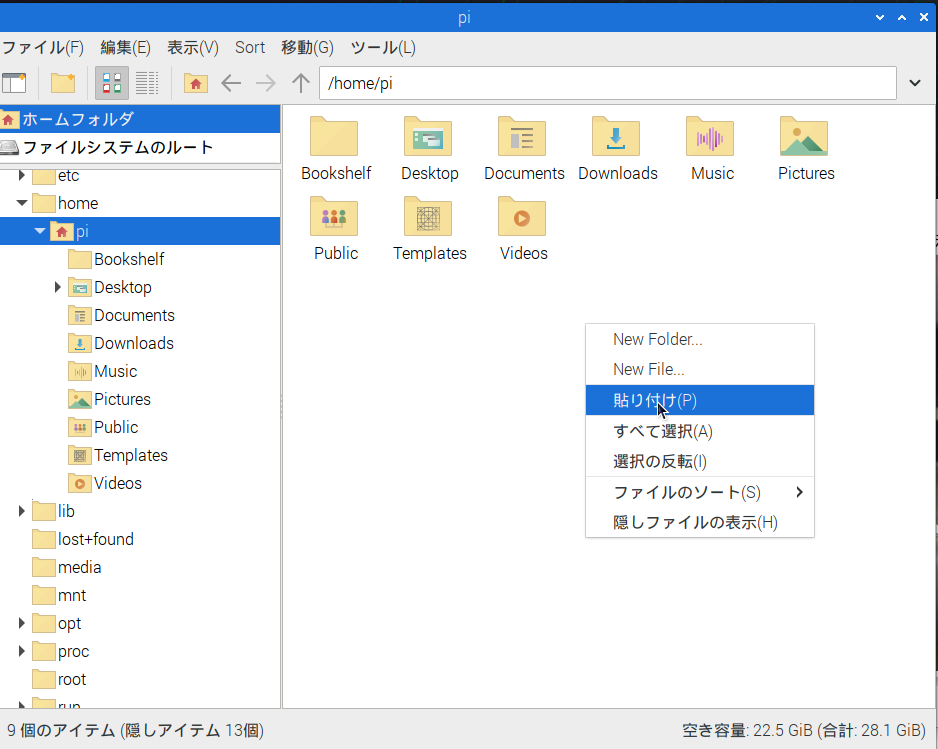
\includegraphics[height=5cm]{../../asset/image/textbook-img1014.png}\\
      \textcircled{\scriptsize{5}} %
      ホームフォルダに\ruby{移動}{いどう}したら、空いているところをクリックして、
      さっきコピーしたフォルダを「\ruby{貼}{は}り付け」ましょう
    \end{minipage}
    \hfill
    \vspace{20pt}
    \begin{minipage}{0.45\linewidth}
      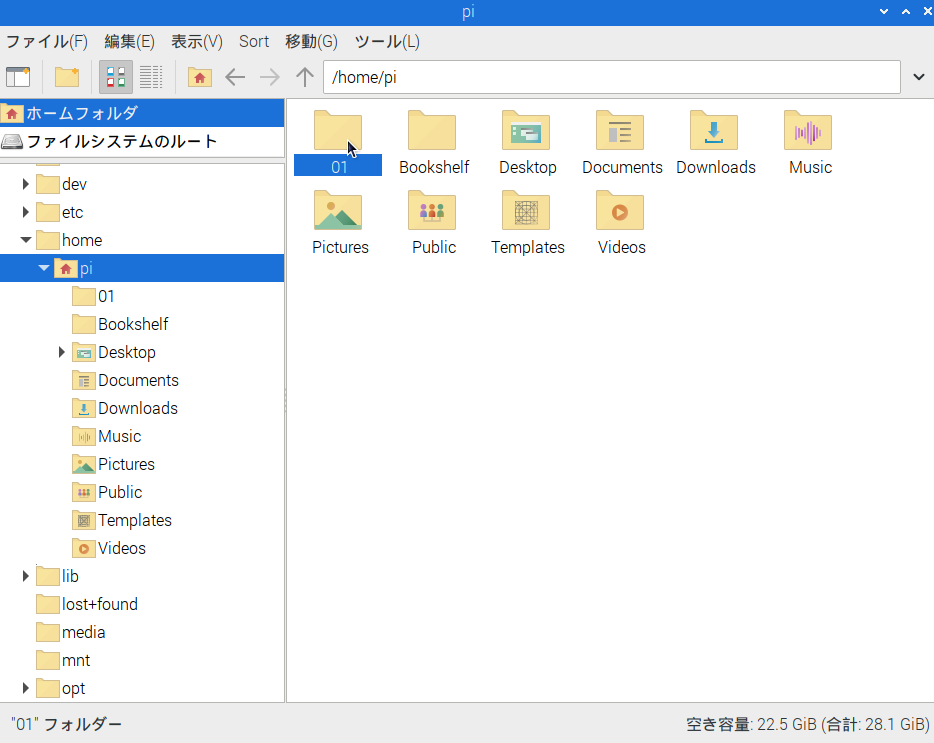
\includegraphics[height=5cm]{../../asset/image/textbook-img1015.png}\\
      \textcircled{\scriptsize{6}} %
      「01」フォルダがあらわれたら、教材の\ruby{準備}{じゅんび}は\ruby{完了}{かんりょう}です
    \end{minipage}

  % \end{minipage}

\clearpage


%
% subsection 1.4.2
%
\subsection{ホームページの中身をのぞいてみよう}


さきほどブラウザでけんさくして見たページを\textbf{ホームページ}（またはウェブページ)といいます。
ホームページを見るにはブラウザを使用しました。
ウェブページのファイル名には、\texttt{.html}(エイチ ティー エム エル)という\ruby{拡張子}{かくちょうし}がついています。
ブラウザはこのhtmlファイルの中身を理解して、ホームページとして\ruby{表示}{ひょうじ}してくれます。
\ruby{自己}{じこ}\ruby{紹介}{しょうかい}ページのテンプレート（先ほどコピーした01フォルダにある
\texttt{self\_intro.html}）の中身をのぞく前に、このファイルをブラウザで開いてみましょう。

\vspace{0.5cm}
\textbf{手順}
\vspace{0.3cm}

まず、ファイルマネージャーで01フォルダを開きます。
赤わくで囲われたところが、以下のようになっていることを\ruby{確認}{かくにん}してください。\\

\texttt{/home/自分のユーザ名/01}\\

\noindent%
以下の\ruby{画像}{がぞう}の場合は、ユーザ名が\texttt{pi}なので、\texttt{/home/pi/01}となっています。
このフォルダ内にある\texttt{self\_intro.html}(黒わくのファイル)をダブルクリックして開きます。

%
\begin{figure}[htbp]
  \centering
  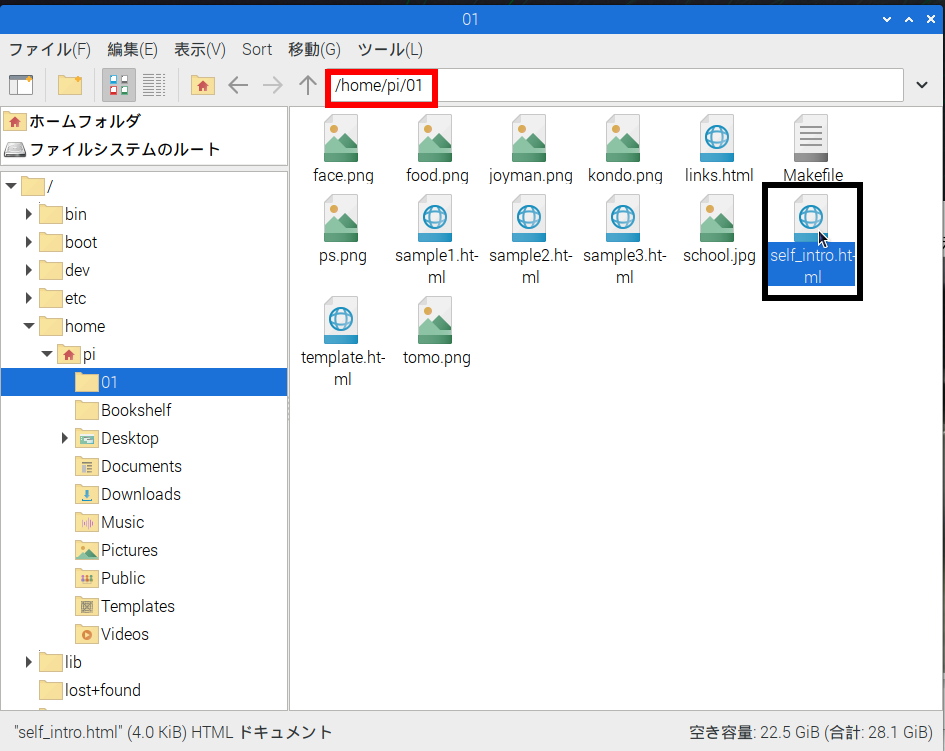
\includegraphics[width=0.8\textwidth]{../../asset/image/textbook-img141.png}
  \caption{htmlファイルを開く}
  \label{fig:1.4.2}
\end{figure}

\clearpage

\noindent%
すると、ブラウザが起動して、以下のようにホームページが\ruby{表示}{ひょうじ}されます。
%
\begin{figure}[htbp]
  \centering
  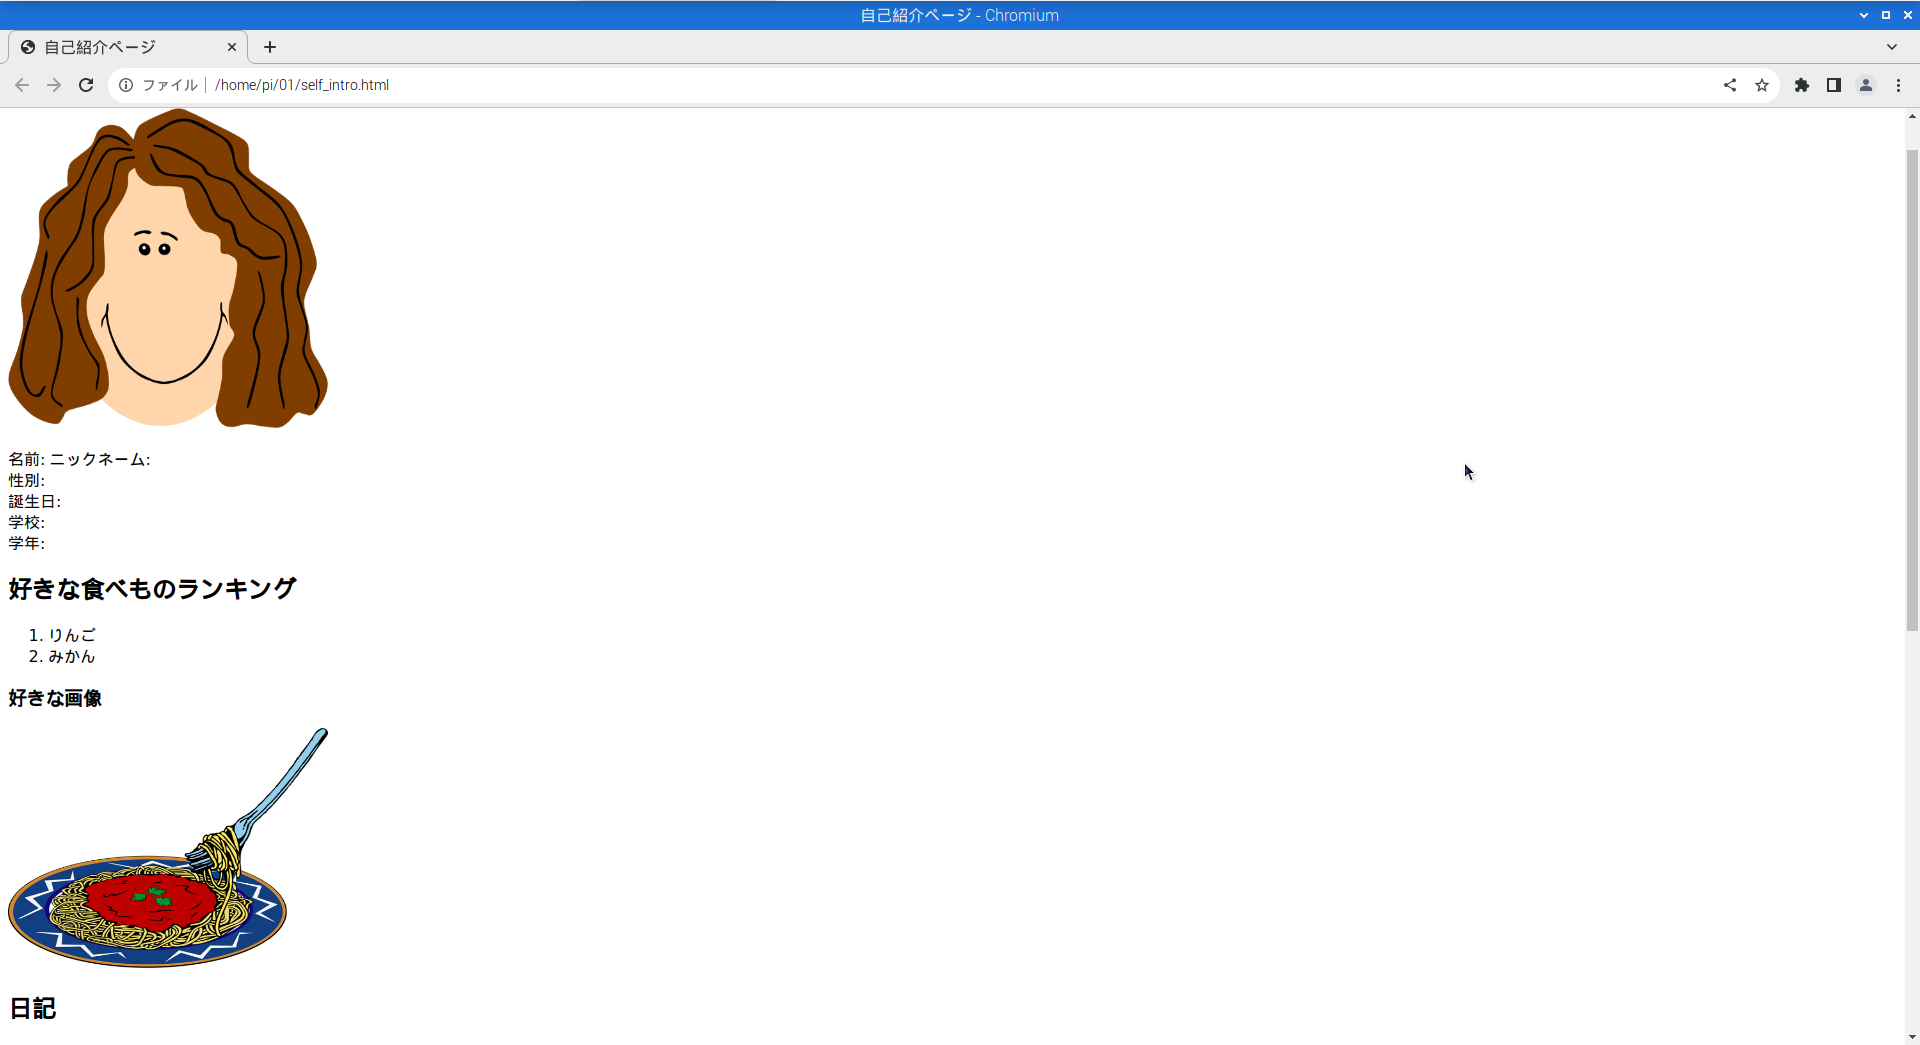
\includegraphics[width=\textwidth]{../../asset/image/textbook-img142.png}
  \caption{ホームページ}
  \label{fig:1.4.3}
\end{figure}


\begin{tcolorbox}[title=\useOmetoi,breakable]
  \begin{enumerate}
    \addex{01フォルダの中にある、\texttt{links.html}をブラウザで開いてみよう。}
  \end{enumerate}
\end{tcolorbox}
\clearpage

%
% subsection 1.4.3
%
\subsection{ホームページの中身を\ruby{編集}{へんしゅう}してみよう}

\indent%
ここでは、\texttt{self\_intro.html}をテキストエディタで開いて、
タイトルバーの文字列を\ruby{変更}{へんこう}してみましょう。
タイトルバーは下の図のように、ブラウザの赤わくの場所に表示されています。
%
\begin{figure}[htbp]
  \centering
  % 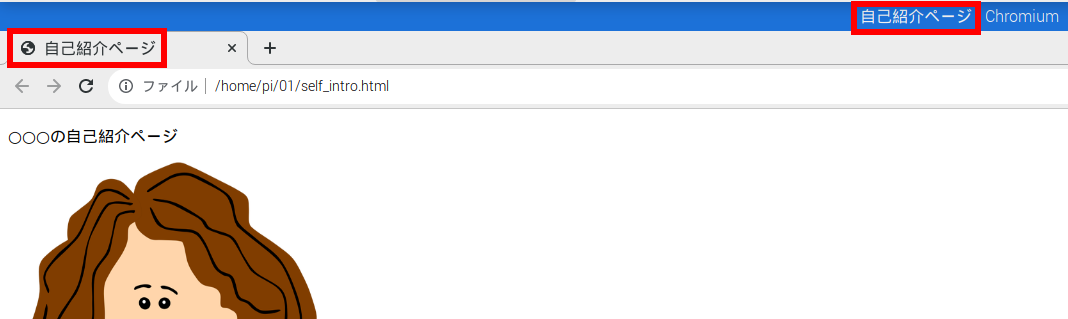
\includegraphics[width=\textwidth]{../../asset/image/textbook-img143.png}
  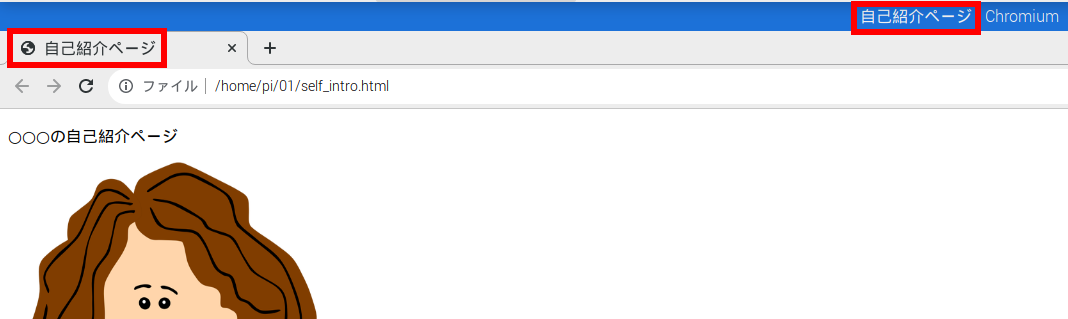
\includegraphics[width=0.9\linewidth]{../../asset/image/textbook-img143.png}
    \caption{ブラウザのタイトル表示}
    \label{fig:1.4.4}
\end{figure}


  
  % \flushleft
  \textbf{手順}
  \vspace{0.3cm}

  % \noindent%
  まずは、Text Editorで\texttt{self\_intro.html}を開いてみましょう。\\
  \vspace{0.5cm}

  % \begin{minipage}{\textwidth}
  \noindent%
    \begin{minipage}{0.45\linewidth}
      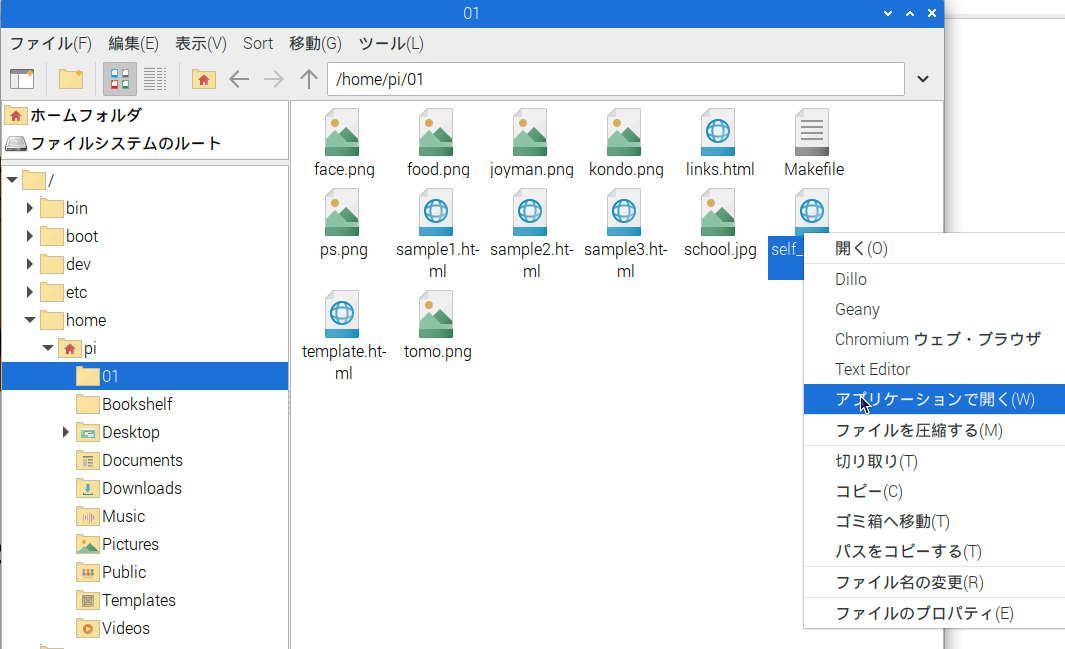
\includegraphics[width=0.9\linewidth]{../../asset/image/textbook-img1040.png}\\
      \textcircled{\scriptsize{1}} %
      \texttt{self\_intro.html}を右クリックして、「アプリケーションで開く」をクリックします
    \end{minipage}
    \hfill
    \vspace{20pt}
    \begin{minipage}{0.45\linewidth}
      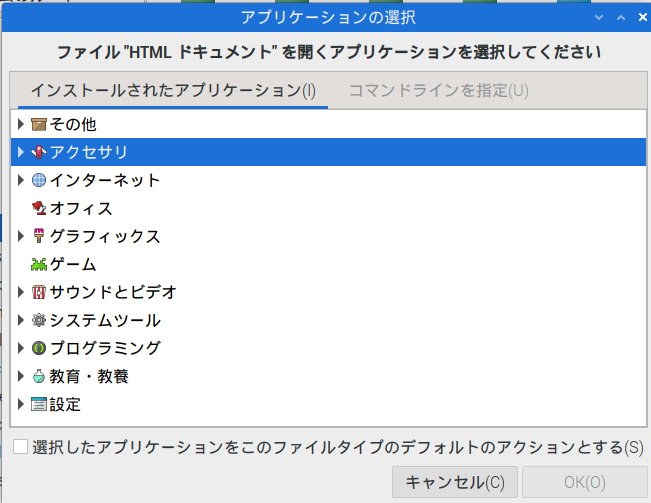
\includegraphics[width=0.9\linewidth]{../../asset/image/textbook-img1041.png}\\
      \textcircled{\scriptsize{2}} %
      「アプリケーションの\ruby{選択}{せんたく}」ウィンドウがでるので、「アクセサリ」をダブルクリックします
    \end{minipage}
    \begin{minipage}{0.45\linewidth}
      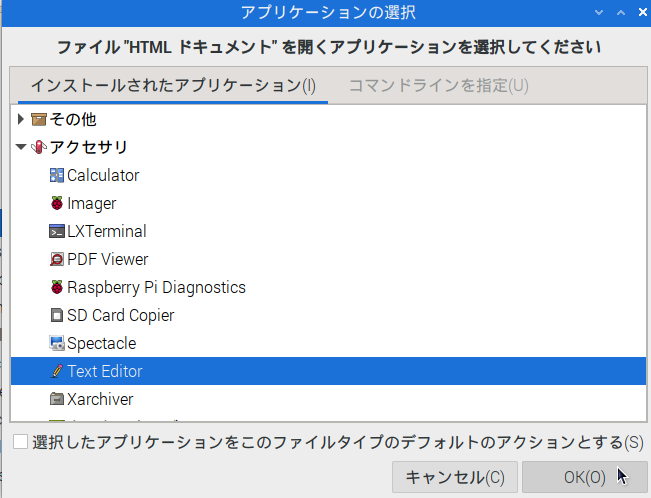
\includegraphics[width=0.9\linewidth]{../../asset/image/textbook-img1042.png}\\
      \textcircled{\scriptsize{3}} %
      「Text Editor」を選んで、OKをクリックします
    \end{minipage}
  % \end{minipage}


% \end{figure}

\clearpage

Text Editorでファイルを開いたら、
\texttt{<title>}\textbf{\ruby{自己}{じこ}\ruby{紹介}{しょうかい}ページ}\texttt{</title>}
を探してください。
ここで、\textbf{\ruby{自己}{じこ}\ruby{紹介}{しょうかい}ページ}を
\textbf{青梅太郎の\ruby{自己}{じこ}\ruby{紹介}{しょうかい}ページ}に\ruby{変更}{へんこう}してみましょう。
青梅太郎は自分の名前に置き\ruby{換}{か}えてください。
\bigskip

\noindent%
\begin{lstlisting}[caption=変更前,label=pwdtest,firstnumber=1]
  <!-- 例題 1-20 ウェブページの中身をのぞいてみよう -->
    <!-- 自己紹介ページ　から　"自分の名前"の自己紹介ページ に変更してみよう -->
    <#red#<title>自己紹介ページ</title>#>
\end{lstlisting}


% \begin{figure}[htbp]
%   \centering
%   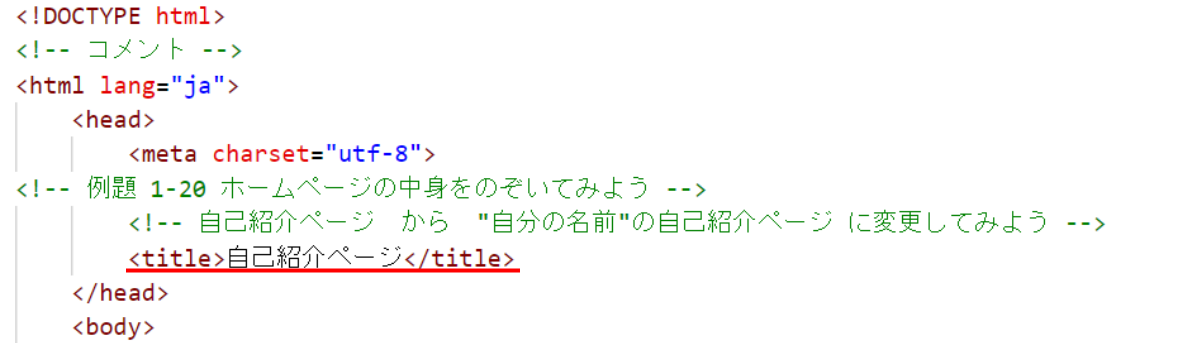
\includegraphics[width=0.9\textwidth]{../../asset/image/textbook-img146.png}
%   \caption{変更前}
%   \label{fig:1.4.5}
% \end{figure}

% \bigskip

\noindent%
以下が、\ruby{変更}{へんこう}した例です。
\bigskip

\noindent%
\begin{lstlisting}[caption=変更後,label=pwdtest,firstnumber=1]
  <!-- 例題 1-20 ウェブページの中身をのぞいてみよう -->
    <!-- 自己紹介ページ　から　"自分の名前"の自己紹介ページ に変更してみよう -->
    <#red#<title>青梅太郎の自己紹介ページ</title>#>
\end{lstlisting}

% \begin{figure}[htbp]
%   \centering
%   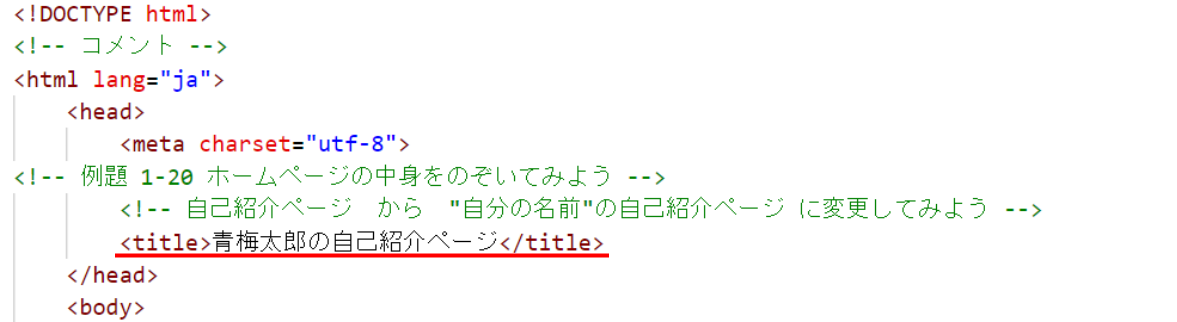
\includegraphics[width=0.9\textwidth]{../../asset/image/textbook-img148.png}
%   \caption{変更後}
%   \label{fig:1.4.6}
% \end{figure}


% \bigskip

\noindent
\ruby{変更}{へんこう}できたら、ファイルを\ruby{保存}{ほぞん}しましょう。
ファイルメニューから\ruby{保存}{ほぞん}を選ぶと、ファイルを上書き\ruby{保存}{ほぞん}することができます。

\begin{figure}[htbp]
  \centering
  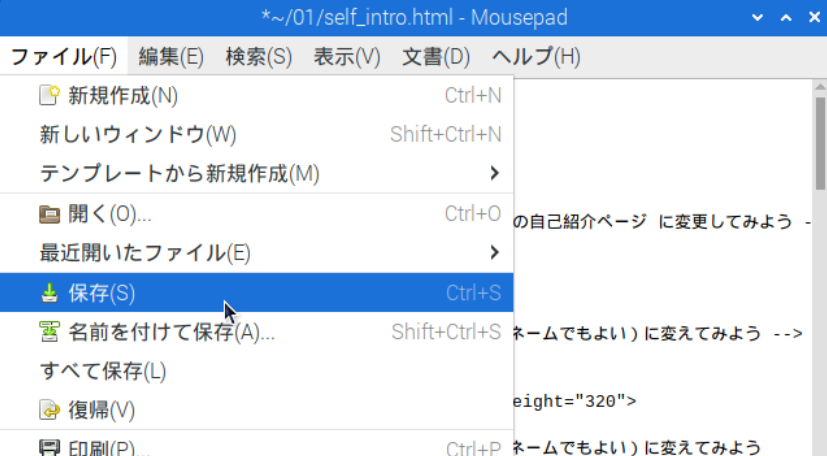
\includegraphics[width=0.7\textwidth]{../../asset/image/textbook-img147.png}
  \caption{ファイルの保存}
  \label{fig:1.4.7}
\end{figure}

\clearpage

ファイルの内容を\ruby{変更}{へんこう}して、\ruby{保存}{ほぞん}しました。
\ruby{変更}{へんこう}した内容をブラウザに\ruby{反映}{はんえい}させるためには、
ブラウザで新しい内容をあらためて読み込む必要があります。
ブラウザでページを読み込み直すことをリロードといいます。
ブラウザの上部に、赤わくで囲われたように、円の形をした矢印（リロードボタン）があります。
これをクリックすることでリロードされ、\ruby{変更}{へんこう}した内容がブラウザに\ruby{反映}{はんえい}されます。

\begin{figure}[htbp]
  \centering
  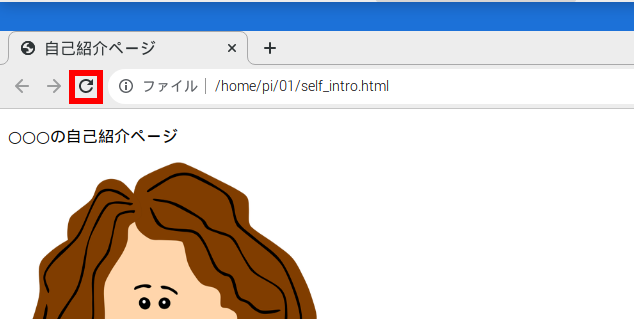
\includegraphics[width=0.7\textwidth]{../../asset/image/textbook-img149.png}
  \caption{リロード}
  \label{fig:1.4.8}
\end{figure}

\texttt{<title>}\textbf{青梅太郎の\ruby{自己}{じこ}\ruby{紹介}{しょうかい}ページ}\texttt{</title>}
と\ruby{変更}{へんこう}した結果、ブラウザのタイトルバー（赤わくで囲われた部分）は、これに\ruby{対応}{たいおう}して
\textbf{青梅太郎の\ruby{自己}{じこ}\ruby{紹介}{しょうかい}ページ}と変わっていることを\ruby{確認}{かくにん}してください。
\ruby{皆}{みな}さんの場合は、自分の名前が\ruby{表示}{ひょうじ}されているはずです。

\begin{figure}[htbp]
  \centering
  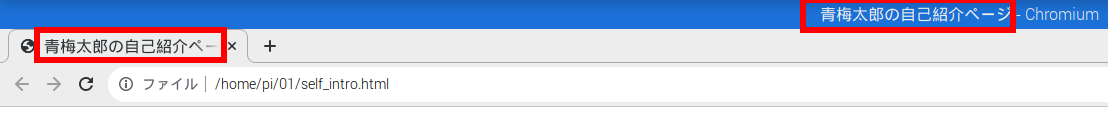
\includegraphics[width=0.8\textwidth]{../../asset/image/textbook-img152.png}
  \caption{タイトルを変更した結果}
  \label{fig:1.4.9}
\end{figure}

% 
% 
% 
\subsubsection{コメントを入れよう}
\hrule\vspace*{5mm}

\texttt{self\_intro.html}の二行目に注目してください。
ここには、

\texttt{<!-- } コメント \texttt{ -->}

\noindent
と書かれています。
これをコメントとよびます。コメントは、内容を分かりやすくするためのメモのようなもので、
ブラウザには\ruby{表示}{ひょうじ}されません。

コメントを入れるには、始まりの記号\texttt{<!--}と終わりの記号\texttt{-->}を使います。
この2つの記号にはさまれた部分がすべてコメントになります。
この2つの記号の間であれば、文章を何行入れても改行しても構いません。

それでは、タイトルバーの文章を変えた行の上に、「\textbf{ここを変えるとタイトルバーも変わる}」
というコメントを追加してみましょう。
\clearpage

\noindent%
\begin{lstlisting}[caption=コメントを追加した例,label=pwdtest,firstnumber=1]
  <!-- 例題 1-20 ウェブページの中身をのぞいてみよう -->
    <!-- 自己紹介ページ　から　"自分の名前"の自己紹介ページ に変更してみよう -->
    <#red#<!-- ここを変えたらタイトルバーも変わる -->#> 
    <title>青梅太郎の自己紹介ページ</title>
\end{lstlisting}

\noindent%
できましたか？
このファイルを良く見てみてください。
このファイルには、コメントがたくさん書いてあります。
そのコメントを読むと、どの場所でどんなことを行っているかが分かると思います。
みなさんも、自分でホームページを作るときには、たくさんのコメントを書いて、
分かりやすくすることを心がけましょう。
\clearpage


%
% subsection 1.4.4
%
\subsection{ホームページの見出しを作ってみよう}

% \indent%
HTMLにかぎらず、見出しを作ることは読みやすい文書を作成するために重要です。
また、改行を\ruby{適切}{てきせつ}に行うことも大切です。

まずは、見出しを作ってみましょう。
ここでは、\textbf{〇〇〇の\ruby{自己}{じこ}\ruby{紹介}{しょうかい}ページ}という見出しを、
自分の名前に\ruby{変更}{へんこう}してみます。

以下の例のように、テキストエディタを使って、〇〇〇を自分の名前に\ruby{変更}{へんこう}します。
\ruby{変更}{へんこう}したら\ruby{保存}{ほぞん}してブラウザをリロードするのを忘れないようにしましょう。
\bigskip

\noindent%
\begin{lstlisting}[caption=見出しを\ruby{変更}{へんこう}した例,label=pwdtest,firstnumber=1]
  <!-- 例題 1-21 見出しを作ってみよう -->
		<!-- 見出しの〇〇〇を自分の名前（ニックネームでもよい）に変えてみよう -->
		<#red#<p>青梅太郎の自己紹介ページ</p>#>
\end{lstlisting}

\begin{figure}[htbp]
  \centering
  % 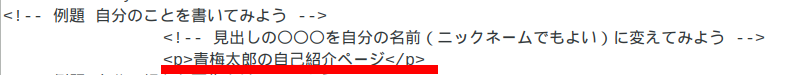
\includegraphics[width=0.9\textwidth]{../../asset/image/textbook-img155.png}\\
  % \mbox{ }\\
  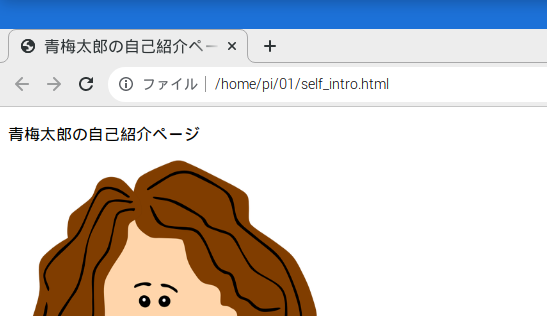
\includegraphics[width=0.7\textwidth]{../../asset/image/textbook-img153.png}
\caption{見出しを\ruby{変更}{へんこう}した例}
  \label{fig:1.4.11}
\end{figure}

見出しとしてはまだ文字が小さく目立たないですね。
それでは、もっと大きくしてみましょう。
% 
% \noindent%
文字を大きくして見出しにするには、

\texttt{<p>}青梅太郎の自己紹介ページ\texttt{</p>}

\noindent%
を以下のように\ruby{変更}{へんこう}します。

\texttt{<h1>}青梅太郎の自己紹介ページ\texttt{</h1>}

\noindent%
\ruby{変更}{へんこう}できたら、保存してブラウザをリロードしてみてください。
今度は、見出しらしく太文字で目立つようになりましたね。
\bigskip

\noindent%
\begin{lstlisting}[caption=見出しを\ruby{変更}{へんこう}した例2,label=pwdtest,firstnumber=1]
  <!-- 例題 1-21 見出しを作ってみよう -->
		<!-- 見出しの〇〇〇を自分の名前（ニックネームでもよい）に変えてみよう -->
		<#red#<h1>青梅太郎の自己紹介ページ</h1>#>
\end{lstlisting}
\clearpage

\begin{figure}[htbp]
  \centering
  % 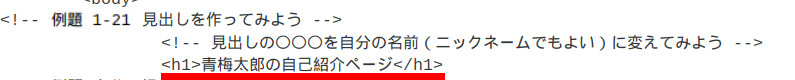
\includegraphics[width=0.9\textwidth]{../../asset/image/textbook-img157.png}\\
  % \mbox{ }\\
  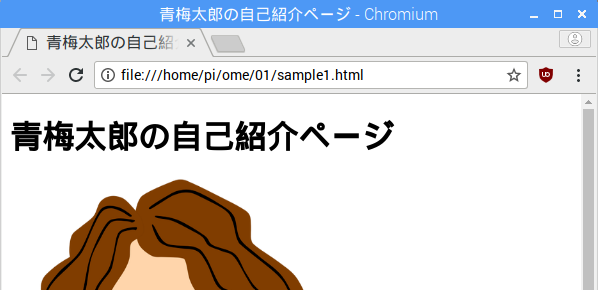
\includegraphics[width=0.7\textwidth]{../../asset/image/textbook-img156.png}
  \caption{見出しを\ruby{変更}{へんこう}した例2}
  \label{fig:1.4.12}
\end{figure}

\texttt{<p>}〇〇〇〇〇\texttt{</p>}や\texttt{<h1>}〇〇〇〇〇\texttt{</h1>}
のように記述されたものを、それぞれ\texttt{p}タグ、\texttt{h1}タグといいます。
また、〇〇〇〇〇の前にある\texttt{<p>}や\texttt{<h1>}は\textbf{開始タグ}、
〇〇〇〇〇の後にある\texttt{</p>}や\texttt{</h1>}は\textbf{\ruby{終了}{しゅうりょう}タグ}とよばれます。
\textbf{タグ}にはそれぞれ\ruby{役割}{やくわり}があって、
タグの間に\ruby{挟}{はさ}まれている文字列（〇〇〇〇〇）にその\ruby{効果}{こうか}があらわれます。

\begin{description}
  \item[pタグ] 文章として\ruby{表示}{ひょうじ}されます。文章を書くときに使用します。
  \item[h1タグ] 見出しとして\ruby{表示}{ひょうじ}されます。見出しを作るときに使用します。
\end{description}

\noindent%
なお、\textbf{タグには半角文字しかつかえません}。
\vspace{0.5cm}

\begin{tcolorbox}[title=\useOmetoi,breakable]
  \begin{enumerate}
    \addex{\texttt{h1}を\texttt{h2}、\texttt{h3}、\texttt{h4}、\texttt{h5}、\texttt{h6}にそれぞれ変えてみて、表示がどう変化するか確かめてみましょう。}
  \end{enumerate}
\end{tcolorbox}
\clearpage




%
% subsection 1.4.5
%
\subsection{\ruby{授業}{じゅぎょう}で使用するタグのいちらん}

ホームページを作るときによく使用するタグを下の表に示します。使い方を例題をつかって学んでいきましょう。

%表作成
\begin{table}[htbp]
  \centering
  \caption{文字タイプ表}
  \footnotesize
  \begin{tabular}{|p{1.3cm}|p{3.9cm}|p{6.3cm}|p{1.5cm}|}
    \hline
      タグ名 & 使用例 & \ruby{効果}{こうか} & 章番号\\
      \hline
      \texttt{title} & \texttt{<title>}タイトル\texttt{</title>} & ブラウザのタイトルバーをタイトルに\ruby{変更}{へんこう}する & 1.4.3\\
      \hline
      \texttt{p} &\texttt{<p>}文章\texttt{</p>} & 文章と\ruby{表示}{ひょうじ}する。改行なし & 1.4.4\\
      \hline
      \texttt{h1} & \texttt{<h1>}見出し１\texttt{</h1>} & 見出し１と\ruby{表示}{ひょうじ}する。\ruby{普通}{ふつう}の文字より大きい & 1.4.4\\
      \hline
      \texttt{img} & \texttt{<img src=”img.png”>} & \texttt{src=""}で指定された\ruby{画像}{がぞう}ファイルを\ruby{表示}{ひょうじ}する & 1.4.6\\
      \hline
      \texttt{br} & \texttt{<br>} & 改行する & 1.4.7\\
      \hline
      \texttt{ol} &
      \begin{tabular}{l}
        \texttt{<ol>}\\
        \ \ \ \texttt{<li>}1位\texttt{</li>}\\
        \texttt{</ol>} 
      \end{tabular}
      & 
      \begin{tabular}{l}
        \texttt{li}タグと合わせて使用する\\
        \ruby{順序}{じゅんじょ}付きのリストを作る\\
        \ruby{順序}{じゅんじょ}番号は\texttt{li}タグの順番通りにつく
      \end{tabular} 
      & 1.4.8\\
      \hline
      \texttt{ul} & 
      \begin{tabular}{l}
        \texttt{<ul>}\\
        \ \ \ \texttt{<li>}\ruby{箇条}{かじょう}書き\texttt{</li>}\\
        \texttt{</ul>} 
      \end{tabular}
      &
      \begin{tabular}{l}
        \ruby{順序}{じゅんじょ}なしのリストを作る\\
        リストは${\bullet}$で始まる 
      \end{tabular} 
      & 1.4.12\\
      \hline
      \texttt{i} & \texttt{<i>}イタリック\texttt{</i>} & 文字を\ruby{斜体}{しゃたい}で\ruby{表示}{ひょうじ}する & 1.4.9\\
      \hline
      \texttt{u} & \texttt{<u>}アンダーライン\texttt{</u>} & 文字に下線を\ruby{表示}{ひょうじ}する & 1.4.9\\
      \hline
      \texttt{strong} &
      \texttt{<strong>}強調\texttt{</strong>}
      & 文字を目立たせる & 1.4.9\\
      \hline
      \texttt{font} &
      \begin{tabular}{l}
        \texttt{<font color="\#019a66">}\\
        \ \ \ 色付き文字\\
        \texttt{</font>}
      \end{tabular}
      & \texttt{color=""}で指定した色で文字を\ruby{表示}{ひょうじ}する & 1.4.9\\
      \hline
      \texttt{font} &
      \begin{tabular}{l}
        \texttt{<font size="1">}\\
        文字の大きさを変える\\
        \texttt{</font>}
      \end{tabular}
      & \texttt{size=""}で指定した文字の大きさで\ruby{表示}{ひょうじ}する & 1.4.9\\
      \hline
      \texttt{table} &
      \begin{tabular}{l}
        \texttt{<table>}\\
        ~\\
        \texttt{</table>}
      \end{tabular}
      & 
      \begin{tabular}{l}
        \texttt{caption}，\texttt{tr}，\texttt{th}，\texttt{td}タグを\\
        使って表を作成する
      \end{tabular}
      & 1.4.10\\
      \hline
      \texttt{caption} & \texttt{<caption>}題\texttt{</caption>} & 表のタイトルを\ruby{表示}{ひょうじ}する & 1.4.10\\
      \hline
      \texttt{tr} & 
      \begin{tabular}{l}
        \texttt{<tr>}\\
        ~\\
        \texttt{</tr>}
      \end{tabular}
      & \texttt{th},\texttt{td}タグを使って表の行を作成する& 1.4.10\\
      \hline
      \texttt{th} & \texttt{<th>}列のタイトル\texttt{</th>} & 表の列のタイトルを\ruby{表示}{ひょうじ}する & 1.4.10\\
      \hline
      \texttt{td} & \texttt{<td>}列のデータ\texttt{</td>} & 表の列のデータを\ruby{表示}{ひょうじ}する & 1.4.10\\
      \hline
      \texttt{a} &
      \begin{tabular}{l}
        \texttt{<a href="google.com">}\\
        \ \ \ google\\
        \texttt{</a>}
      \end{tabular}
      & 
      \begin{tabular}{l}
        クリックすると登録していたホームページに\\
        \ruby{移動}{いどう}するリンクを作成する
      \end{tabular}
       & 1.4.11\\
      \hline
  \end{tabular}
\end{table}

\clearpage




%
% subsection 1.4.6
%
\subsection{自分の好きな\ruby{画像}{がぞう}をホームページにはってみよう}


% %\begin{figure}[ht]
% \flushleft
% \subsection{例題 1-22 自分の好きな\ruby{画像}{がぞう}をはってみよう}

ホームページには、自分のお気に入りの画像をはりつけて、表示させることができます。
ここでは、練習として、前章でウェブカメラを使って\ruby{撮影}{さつえい}した
自分の写真を表示させてみましょう。


\textbf{手順}
\vspace{0.5cm}

まずは、表示させたい\ruby{画像}{がぞう}を、\texttt{self\_intro.html}があるフォルダと同じ場所にコピーします。
\vspace{0.5cm}


\noindent%
\begin{minipage}{0.45\linewidth}
  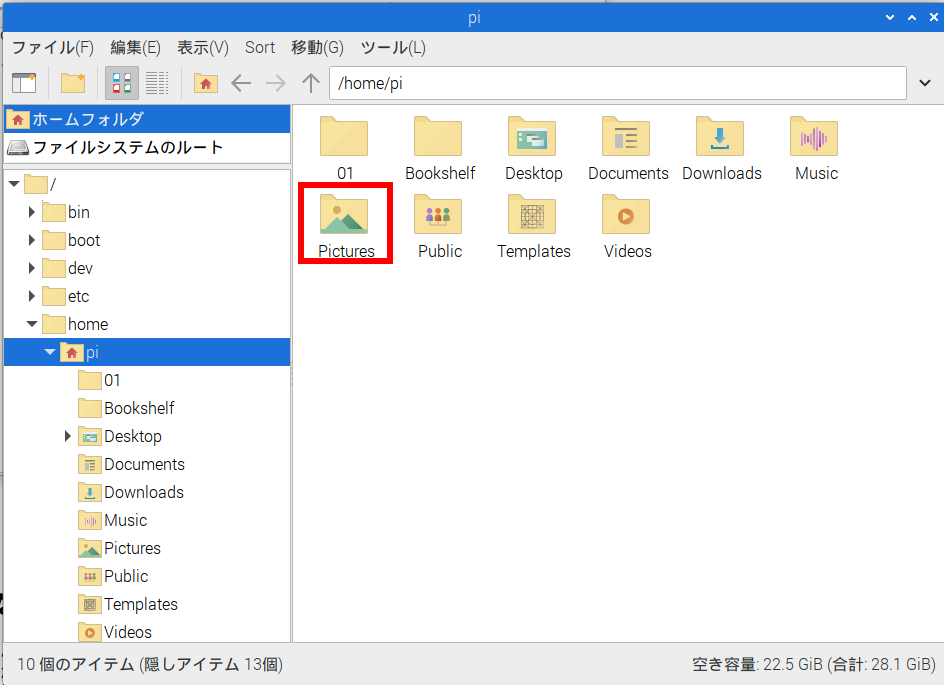
\includegraphics[width=0.9\linewidth]{../../asset/image/textbook-img164.png}\\
  \textcircled{\scriptsize{1}} %
  Picturesをダブルクリックします
\end{minipage}
\hfill
\vspace{20pt}
\begin{minipage}{0.45\linewidth}
  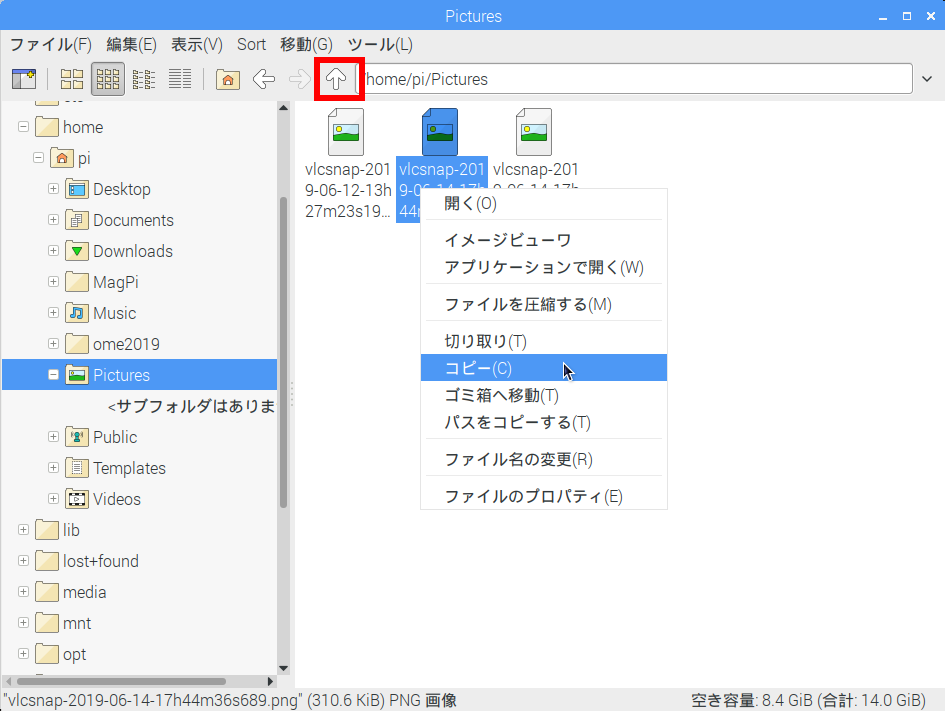
\includegraphics[width=0.9\linewidth]{../../asset/image/textbook-img163.png}\\
  \textcircled{\scriptsize{2}} %
  使いたい\ruby{画像}{がぞう}の上で右クリックして、コピーを選択したあとで、赤枠の上矢印をクリックします
\end{minipage}
%
\begin{minipage}{0.45\linewidth}
  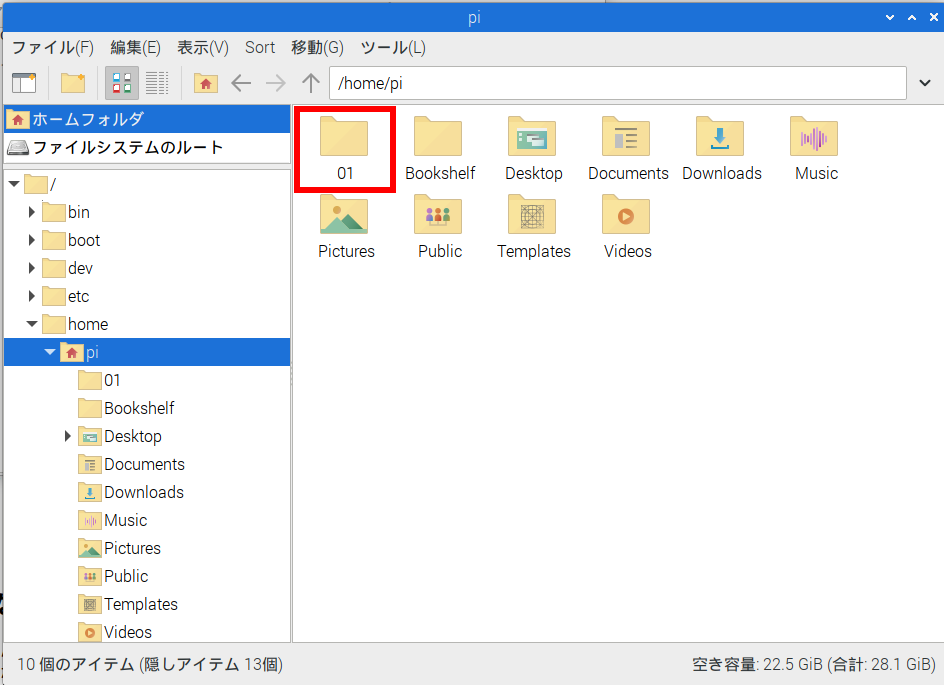
\includegraphics[width=0.9\linewidth]{../../asset/image/textbook-img167.png}\\
  \textcircled{\scriptsize{3}} %
  01フォルダをダブルクリックします
\end{minipage}
\hfill
\vspace{20pt}
\begin{minipage}{0.45\linewidth}
  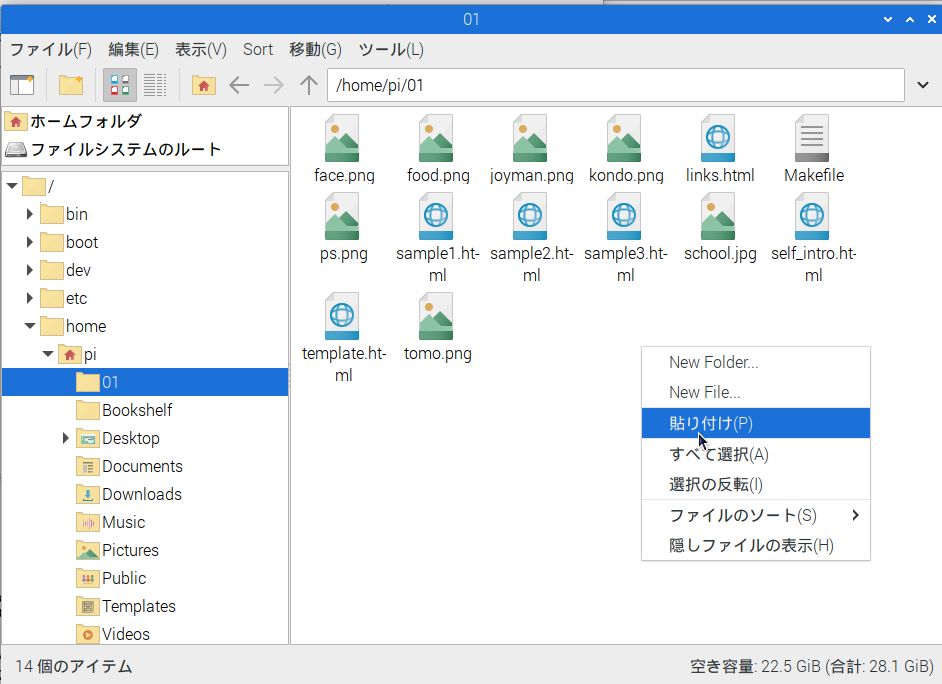
\includegraphics[width=0.9\linewidth]{../../asset/image/textbook-img168.png}\\
  \textcircled{\scriptsize{4}} %
  右クリックして\ruby{貼}{は}り付けを\ruby{選択}{せんたく}します
\end{minipage}
%
\begin{minipage}{0.45\linewidth}
  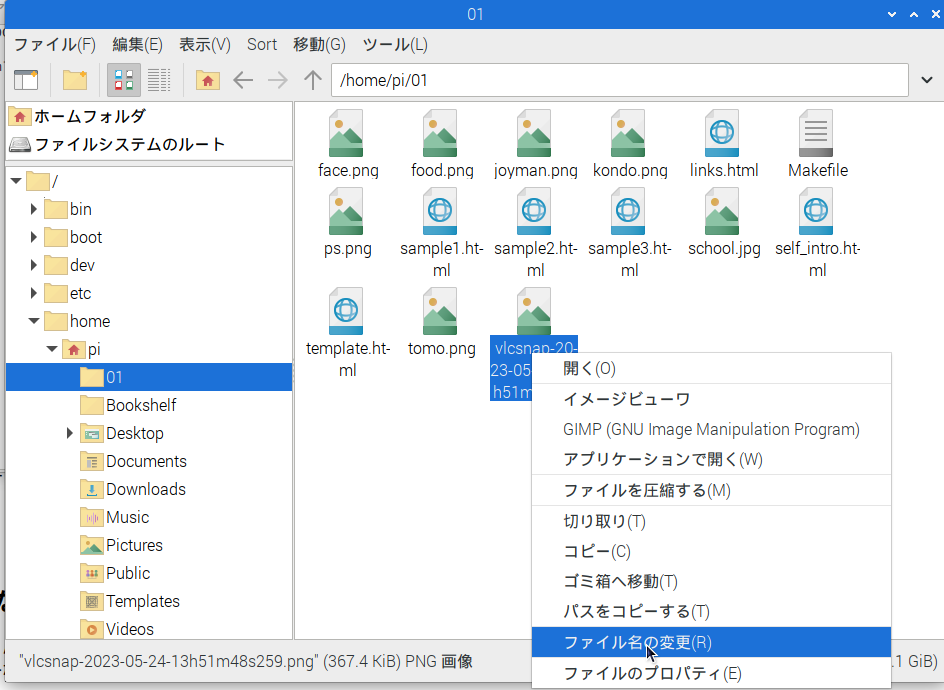
\includegraphics[width=0.9\linewidth]{../../asset/image/textbook-img169.png}\\
  \textcircled{\scriptsize{5}} %
  \ruby{貼}{は}り付けたファイルを右クリックして、「ファイル名の\ruby{変更}{へんこう}」を選択します
\end{minipage}
\hfill
\vspace{20pt}
\begin{minipage}{0.45\linewidth}
  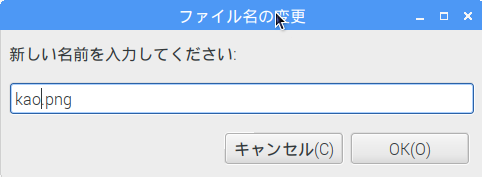
\includegraphics[width=0.9\linewidth]{../../asset/image/textbook-img166.png}\\
  \textcircled{\scriptsize{6}} %
  ここでは\texttt{kao.png}に\ruby{変更}{へんこう}しましょう
\end{minipage}
\clearpage


\ruby{画像}{がぞう}のコピーができたら、次にhtmlファイルを\ruby{編集}{へんしゅう}して、
\ruby{自己}{じこ}\ruby{紹介}{しょうかい}ページに\ruby{表示}{ひょうじ}しましょう。
次のリストの2行目が\ruby{画像}{がぞう}を\ruby{表示}{ひょうじ}するためのタグです。
\bigskip


\noindent%
\begin{lstlisting}[caption=\ruby{画像}{がぞう}の表示,label=pwdtest,firstnumber=1]
    <!-- 例題 1-22 自分の好きな画像をはってみよう -->
    <#red#<img src="face.png" width="320" height="320">#> 
\end{lstlisting}

\noindent%
このimgタグで使われているパラメータには、それぞれ以下のような意味があります。

\begin{description}
  \item[\texttt{href=""}]  表示する画像ファイルを指定する
  \item[\texttt{width=""}]  画像の幅を指定する
  \item[\texttt{height=""}]  画像の高さを指定する
\end{description}

\noindent%
つまり、このタグは、ファイル\texttt{face.png}の画像を、横幅320ピクセル、高さ320ピクセルの大きさで表示することを表しています。
それでは、このタグを\ruby{編集}{へんしゅう}して、さきほどコピーしたファイル\texttt{kao.png}の画像を表示させてみましょう。
\bigskip


\begin{lstlisting}[caption=\ruby{画像}{がぞう}の表示（\ruby{編集}{へんしゅう}後）,label=pwdtest,firstnumber=1]
  <!-- 例題 1-22 自分の好きな画像をはってみよう -->
  <#red#<img src="kao.png" width="320" height="320">#> 
\end{lstlisting}


\noindent%
上の例のように変更して、ブラウザをリロードすると、写真が表示されます。
\bigskip


\begin{tcolorbox}[title=\useOmetoi,breakable]
  \begin{enumerate}
    \addex{スパゲッティの\ruby{画像}{がぞう}をウェブカメラでとった\ruby{画像}{がぞう}（教室の風景など）に変更してみましょう。}
    ヒント
    \begin{enumerate}
      \item まず、\ruby{画像}{がぞう}を01フォルダの中にコピーして名前を\ruby{変更}{へんこう}しましょう。
      \item 次に、imgタグの\ruby{画像}{がぞう}ファイル名を、コピーしたファイル名に\ruby{変更}{へんこう}しましょう。
    \end{enumerate} 
    \vspace{0.5cm}
    \addex{この\ruby{画像}{がぞう}が表示される大きさを変更してみましょう。大きさを変えるには、\texttt{width}と\texttt{height}の値を\ruby{変更}{へんこう}します。}
  \end{enumerate}
\end{tcolorbox}
\clearpage



%
% subsection 1.4.7
%
\subsection{ウェブページで自分のことを\ruby{紹介}{しょうかい}しよう}

ここでは、自分のことを紹介するページを作成します。
まずは今回\ruby{変更}{へんこう}するページをブラウザで見てみましょう。

\begin{figure}[htbp]
  \centering
  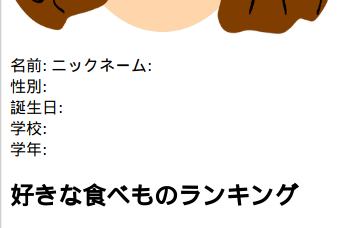
\includegraphics[width=0.5\textwidth]{../../asset/image/textbook-img175.png}
  \caption{\ruby{紹介}{しょうかい}ページ（\ruby{編集}{へんしゅう}前）}
  \label{fig:1.4.15}
\end{figure}

\noindent%
このままでは、「名前：」と「ニックネーム：」が同じ行に表示されてしまっています。
まずは、改行の仕方を学びましょう。
テキストエディタへ\ruby{戻}{もど}ってください。
文章中で改行するためにはbrタグを使用します。\\
\texttt{<br>}\\
ウェブページは、brタグを\ruby{挿入}{そうにゅう}した位置で改行されます。
なお、このbrタグには\ruby{終了}{しゅうりょう}タグがありませんので気を付けてください。
次のリストの8行目のように、コメント行の下に\texttt{<br>}タグを\ruby{挿入}{そうにゅう}してみてください。
\bigskip

% \begin{figure}[htbp]
%   \centering
%   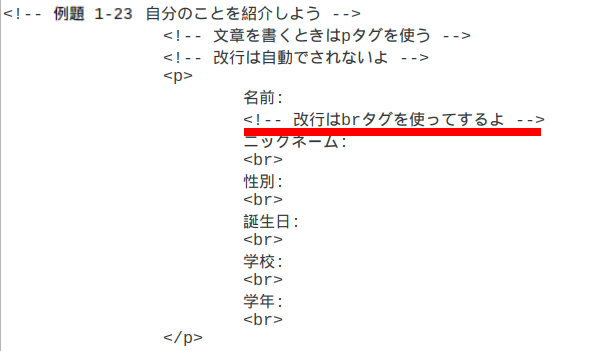
\includegraphics[width=0.5\textwidth]{../../asset/image/textbook-img174.png}
%   \caption{\ruby{紹介}{しょうかい}ページ（\ruby{編集}{へんしゅう}前）}
%   \label{fig:1.4.16}
% \end{figure}

\begin{lstlisting}[caption=\ruby{紹介}{しょうかい}ページ（\ruby{編集}{へんしゅう}後）,label=pwdtest,firstnumber=1]
  <!-- 例題 1-23 自分のことを紹介しよう -->
		<!-- 見出しの〇〇〇を自分の名前（ニックネームでもよい）に変えてみよう 
		文章を書くときはpタグを使う 
		改行は自動でされないよ -->
		<p>
			名前: 
			<#red#<!-- 改行はbrタグを使ってするよ -->#>
			<#blue#<br>#>
			ニックネーム: 
			<br>
			性別: 
			<br>
			誕生日: 
			<br>
			学校: 
			<br>
			学年: 
			<br>
		</p>

\end{lstlisting}


\noindent%
変更したら、ブラウザをリロードして、ページを確認してみましょう。
これで、見やすくなったと思います。
% \clearpage

\begin{figure}[htbp]
  \centering
  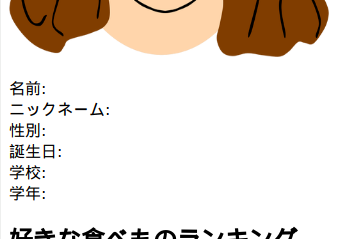
\includegraphics[width=0.5\textwidth]{../../asset/image/textbook-img176.png}
  \caption{\ruby{紹介}{しょうかい}ページ（改行した後）}
  \label{fig:1.4.17}
\end{figure}


次は自分のことを\ruby{紹介}{しょうかい}する内容に書きかえましょう。
名前、\ruby{性別}{せいべつ}、\ruby{誕生日}{たんじょうび}、学校、学年を追加してください。

\begin{figure}[htbp]
  \centering
  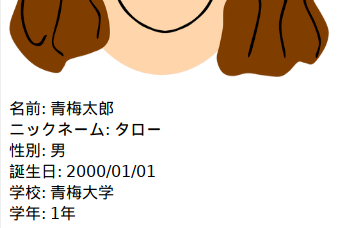
\includegraphics[width=0.5\textwidth]{../../asset/image/textbook-img173.png}
  \caption{\ruby{紹介}{しょうかい}ページの例}
  \label{fig:1.4.18}
\end{figure}



\begin{tcolorbox}[title=\useOmetoi,breakable]
  \begin{enumerate}
    \addex{他にも\ruby{紹介}{しょうかい}\ruby{項目}{こうもく}を追加してみましょう（しゅみ、好きなもの、．．．）。}
  \end{enumerate}
\end{tcolorbox}
\clearpage




%
% subsection 1.4.8
%
\subsection{ランキングを作ろう}

自分の好きなことを\ruby{紹介}{しょうかい}するために、ランキングトップ３を作ります。
まずは、ブラウザで見てみましょう。

\begin{figure}[htbp]
  \centering
  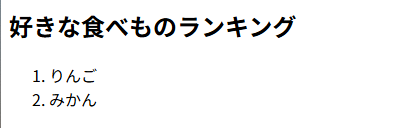
\includegraphics[width=0.6\textwidth]{../../asset/image/textbook-img178x.png}
  \caption{好きな食べ物ランキング}
  \label{fig:1.4.19}
\end{figure}


はじめに、見出しを\ruby{変更}{へんこう}しましょう。\textbf{好きな食べものランキングトップ３}\\に変えてください。
\bigskip

\noindent%
\begin{lstlisting}[caption=見出しの変更,label=pwdtest,firstnumber=1]
  <!-- 例題 1-24 ランキングを作ろう -->
  <#red#<h2>好きな食べものランキングトップ3</h2>#>
\end{lstlisting}

ランキング（順序付きリスト）を作るには、順序付きリストタグ\texttt{<ol>}～\texttt{</ol>}と
リストタグ\texttt{<li>}～\texttt{<li>}を使います。
使用例を、テキストエディタで見てみましょう。
\bigskip

\noindent%
\begin{lstlisting}[caption=順序付きリストの例,label=pwdtest,firstnumber=1]
  <!-- 例題 1-24 ランキングを作ろう -->
  <h2>好きな食べものランキングトップ3</h2>
  <!-- 番号付きのリストを作るときはolタグを使うよ -->
  <#red#<ol>#>
    <!-- リストの中身はliタグで作るよ 
    上から順番に番号がつけられる -->
    <#blue#<li>#>りんご<#blue#</li>#>
    <#blue#<li>#>みかん<#blue#</li>#>
  <#red#</ol>#>
\end{lstlisting}

このように、順序付きリストタグ\texttt{<ol>}～\texttt{</ol>}の中に、
リストタグ\texttt{<li>}～\texttt{<li>}で囲まれた文字列（りんごとみかん）が
入力されています。
実際に、ブラウザでは次の図のように表示されます。
このように、\texttt{<ol>}タグの中で、\texttt{<li>}タグを使って指定された文字列が、
上から順序良く番号付きでリスト表示されていることが分かると思います。
\clearpage

\begin{figure}[htbp]
  \centering
  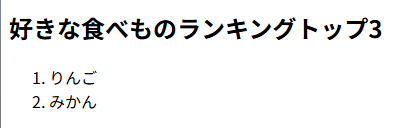
\includegraphics[width=0.6\textwidth]{../../asset/image/textbook-img182x.png}
  \caption{ランキングの表示}
  \label{fig:1.4.20}
\end{figure}


3番目に「ぶどう」が表示されるように、「みかん」の下の行にリストを追加してみましょう。
\bigskip

\noindent%
\begin{lstlisting}[caption=順序付きリストに「ぶどう」を追加した例,label=pwdtest,firstnumber=1]
  <!-- 番号付きのリストを作るときはolタグを使うよ -->
  <ol>
    <!-- リストの中身はliタグで作るよ 
    上から順番に番号がつけられる -->
    <li>りんご</li>
    <li>みかん</li>
    <#red#<li>ぶどう</li>#>
  </ol>
\end{lstlisting}

\noindent%
これで3番目に「ぶどう」が表示されます。
\bigskip

\begin{figure}[htbp]
  \centering
  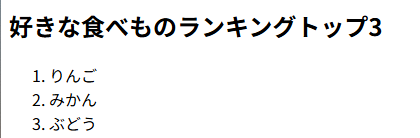
\includegraphics[width=0.6\textwidth]{../../asset/image/textbook-img182xx.png}
  \caption{ぶどうを追加した表示例}
  \label{fig:1.4.20x}
\end{figure}

\begin{tcolorbox}[title=\useOmetoi,breakable]
  \begin{enumerate}
    \addex{好きな食べ物ランキングを実際に好きな食べものに変えてみましょう。}
    \addex{新しいランキングを追加してみましょう（好きなおかしランキング、好きなゲームランキング、．．．）}
  \end{enumerate}
\end{tcolorbox}
\clearpage



%
% subsection 1.4.9
%
\subsection{日記を書いてみよう}

この教室で学んだことや、学校で楽しかったことなどを\ruby{紹介}{しょうかい}してみましょう。
ここでは、より楽しく見える日記にするために、文字の太さや色を変えたり、ななめ文字にしたり、
アンダーラインを引いたり、文字を\ruby{装飾}{そうしょく}する方法について学びましょう。

復習になりますが、文章を書くときには、pタグを使います。
より詳しく説明すると、\texttt{<p>}～\texttt{</p>}で囲まれた文章が、1つの段落（ひとかたまりの文章）になります。
次の例では、日付や日記の本文が段落になっています。
\bigskip

\noindent%
\begin{lstlisting}[caption=段落の例,label=pwdtest,firstnumber=1]
  <!-- 例題 1-18 日記を書いてみよう -->
  <h2>日記</h2>
  <!-- 日記の題名 -->
  <h4>プログラミング教室</h4>
  <#red#<p>#>2025/06/21<#red#</p>#>
  <!-- 日記の本文 -->
  <#red#<p>#>
    自己紹介ページの作り方をべんきょうしている
  <#red#</p>#>
\end{lstlisting}

次に、文字の\ruby{装飾}{そうしょく}について見てみましょう。
\bigskip

\noindent%
\begin{lstlisting}[caption=文字の\ruby{装飾}{そうしょく},label=pwdtest,firstnumber=1]
  <!-- 斜めの文字 -->
  <#red#<i>#>イタリック<#red#</i>#>
  <br>
  <!-- 下線付きの文字 -->
  <#red#<u>#>アンダーライン<#red#</u>#>
  <br>
  <!-- 太文字 -->
  <#red#<strong>#>あいうえお<#red#</strong>#>
  <br>
  <!-- 色付きの文字 -->
  <#red#<font color="#019a66">#>色文字<#red#</font>#>	
  <br>
  <!-- 文字の大きさを変える -->
  <#red#<font size="1">#>文字の大きさ<#red#</font>#>
\end{lstlisting}


ここで使われているタグについて説明します。

\begin{description}
  \item[\texttt{<i>}～\texttt{</i>}]\mbox{}\\
  囲まれた文字列をななめ文字（イタリック体）で表示します
  \item[\texttt{<ul>}～\texttt{</ul>}] \mbox{}\\
  囲まれた文字列の下に線（アンダーライン）を引きます
  \item[\texttt{<strong>}～\texttt{</strong>}] \mbox{}\\
  囲まれた文字列を太字にします
\end{description}

\noindent%
文字のサイズを変えたり，色を付けたりするには、fontタグを使用します。
色は、color属性を使って指定します。
\bigskip

\texttt{<font color="\#RRGGBB">}色を付けたい文字\texttt{</font>}\\
\bigskip

\noindent%
ここで、色はRR（赤の明るさ）GG（緑の明るさ）BB（青の明るさ）を，それぞれ00からFFの16進数で指定します。
例えば、赤は\texttt{"\#FF0000"}、青は\texttt{"\#00FF00"}、緑は\texttt{"\#0000FF"}、
白は\texttt{"\#FFFFFF"}、黒は\texttt"{\#000000"}になります。

\begin{description}
  \item[16進数]\mbox{}\\
  0～9、A～Fの16種類の記号を用いて、1\ruby{桁}{けた}を16この記号（数値）で表したものです。
  例えば、普段使っている数字（10進数）の10は、16進数ではAになります（11はB、12はC、13はD、14はE、15はF、16は10）。
  16進数のFFは10進数では255になります。
\end{description}

このままでは分かりにくいかもしれませんので、色の例を見てみましょう。
\textbf{\ruby{授業}{じゅぎょう}で使用したホームページ\url{links.html}}の2番目にある
\textbf{色の見本}をクリックして開いて見てください。
2番を開くと地下鉄で使っている色の見本が出てきます。
\ruby{銀座線}{ぎんざせん}オレンジは\texttt{\#f39700}となっています。
この値を使って、上のcolorの\ruby{値}{あたい}を\texttt{"\#f39700"}に変えることもできます。
このように\ruby{数値}{すうち}によって\ruby{表示}{ひょうじ}する色を選びます。

\begin{figure}[htbp]
  \centering
  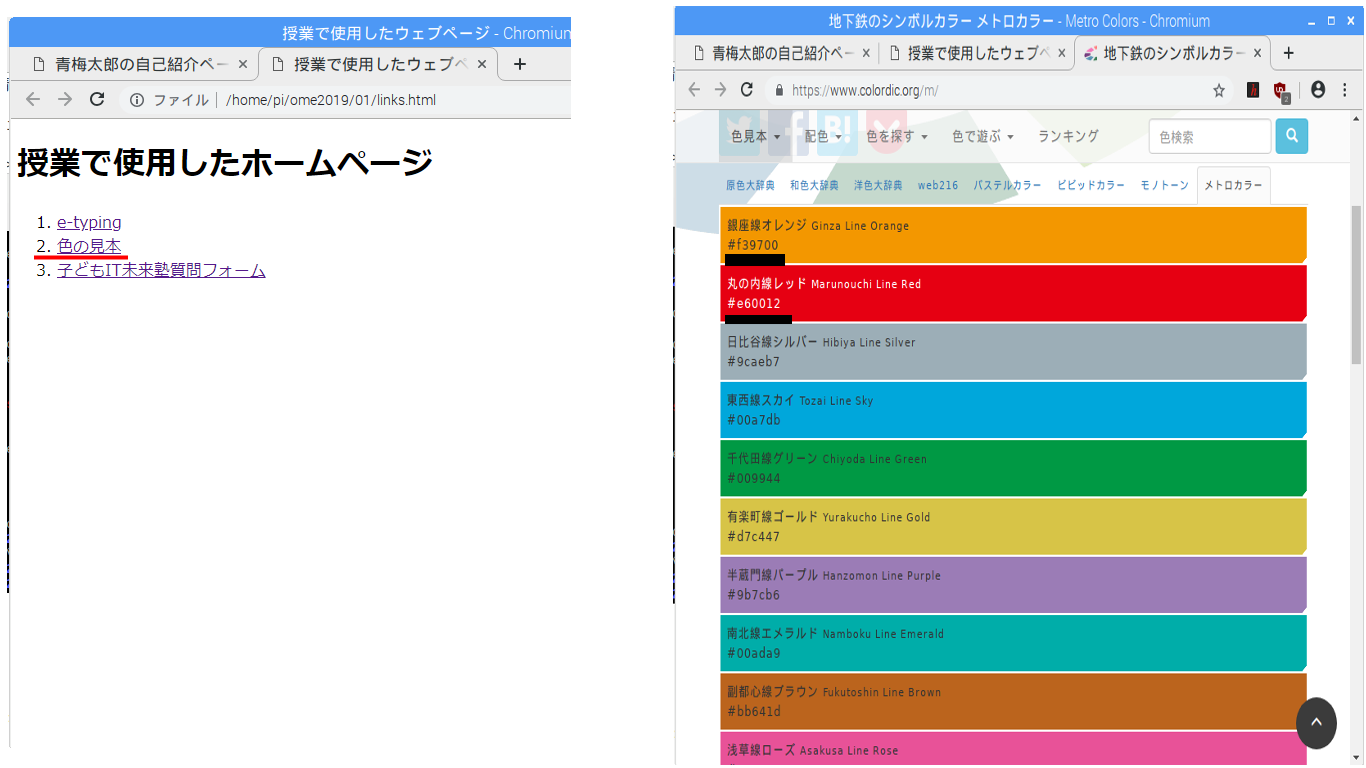
\includegraphics[width=0.95\textwidth]{../../asset/image/textbook-img187.png}
  \caption{色の見本}
  \label{fig:1.4.21}
\end{figure}



\indent%
文字の大きさは、fontタグのsize属性を使って指定します。
\bigskip

\texttt{<font size="1">}大きさをかえたい文字\texttt{</font>}\\
\bigskip

\noindent%
\texttt{size="1"}この数字の1の値を変えると文字のサイズが変化します。
実際に他の数字に変えて、大きさがどうなるか確認してください。

\noindent%
ここで説明したfontタグのcolor属性とsize属性は、同時に使うこともできますので、
いろいろと試してみるのも楽しいと思います。
\bigskip

\texttt{<font color="\#f39700" size="3">}大きいフォントの銀座線オレンジ\texttt{</font>}
\bigskip

最後に、ここで学んだタグを使って、下の例を参考に自分の日記を書いてみましょう。

\begin{figure}[htbp]
  \centering
  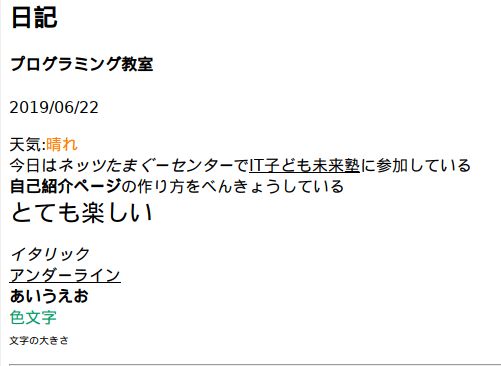
\includegraphics[width=0.7\textwidth]{../../asset/image/textbook-img185.png}
  \caption{日記の例}
  \label{fig:1.4.22}
\end{figure}

\begin{tcolorbox}[title=\useOmetoi,breakable]
  \begin{enumerate}
    \addex{\texttt{<hr>}タグを使うと、ページに横線を引くことができます。日記の一番下に横線を引いてみましょう。}
    \addex{日記を追加してみましょう（ヒント：タイトル、日付、本文の順に追加しましょう）。}
  \end{enumerate}
\end{tcolorbox}
\clearpage



%
% subsection 1.4.10
%
\subsection{グループのメンバー表を作ろう}

ここでは、下の図のように、グループの友だちのことを表にまとめてみましょう。

\begin{figure}[htbp]
  \centering
  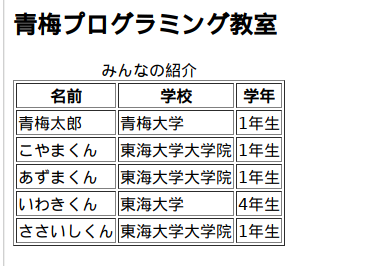
\includegraphics[width=0.5\textwidth]{../../asset/image/textbook-img189.png}
  \caption{メンバー表の例}
  \label{fig:1.4.23}
\end{figure}

表の作成には、tableタグ\texttt{<table>}～\texttt{</table>}を使います。
tabelタグの中に、表の行を作成するtr（Table Row）タグ\texttt{<tr>}～\texttt{</tr>}や、
行の見出しを作成するth（Table Header）タグ\texttt{<th>}～\texttt{</th>}、
行の内容を作成するtd（Table Data）タグ\texttt{<td>}～\texttt{</td>}を入力することで、
表を完成させます。
また、表の見出しの作成にはcaptionタグ\texttt{<caption>}～\texttt{</caption>}を使います。
次に、リストと実際に表示される例を示します。
\bigskip

%
\begin{minipage}{0.58\linewidth}
  \begin{lstlisting}[caption=表の例,label=pwdtest,firstnumber=1]
    <!-- 例題 1-26 グループのメンバー表を作ろう -->
    <h2>青梅プログラミング教室</h2>
    <!-- 表を作るタグ -->
    <#purple#<table border="1">#>
      <!-- 表のタイトル -->
      <#blue#<caption>みんなの紹介</caption>#>
      <!-- 表の行を作るタグ -->
      <#green#<tr>#>
        <!-- 表の列の見出しを作るタグ -->
        <#green#<th>名前</th>
        <th>学校</th>
        <th>学年</th>
      </tr>#>
      <#magenta#<tr>#>
        <!-- 表の列を作るタグ -->
        <#magenta#<td>0くん</td>
        <td>c中学校</td>
        <td>1年生</td>
      </tr>#>
        ・
        ・
        ・
    <#purple#</table>#>
  \end{lstlisting} 
\end{minipage}
\hfill
% 
\vspace{20pt}
\begin{minipage}{0.36\linewidth}
  \centering
  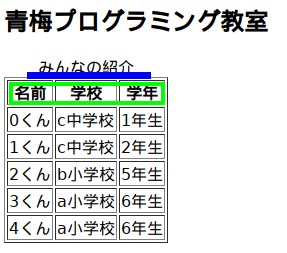
\includegraphics[width=0.95\linewidth]{../../asset/image/textbook-img190x.png}
  \vspace{1cm}

  {\bf 表の作成に使用するタグ}
  \begin{description}
    \item[table]表の作成
    \item[caption]表のタイトル
    \item[tr]行の作成
    \item[th]行の見出しの作成
    \item[td]行の内容の作成
  \end{description}
\end{minipage}

\clearpage

表を作成するためには、tableタグ\texttt{<table>}～\texttt{</table>}の中に、
各要素を書いていきます。今回の例では，
\bigskip

\begin{lstlisting}[caption=表の作成,label=pwdtest,firstnumber=1]
  <table border="1">
     ・
     ・
  </table>
\end{lstlisting} 

\noindent%
のように、border属性が使われています。
これは、表の枠の太さを決める値です。
ここでは、太さが1の枠で仕切られた表が表示されることになります。

表にタイトルを付けるためには、captionタグを使用します。
\bigskip
\begin{lstlisting}[caption=表のタイトル,label=pwdtest,firstnumber=1]
    <!-- 表のタイトル -->
    <caption>みんなの紹介</caption>
\end{lstlisting} 
\noindent%
ここで指定している「みんなの紹介」というタイトルは、表の上部に表示されます。

表は、行ごとに作成します。
表の行の作成にはtrタグ\texttt{<tr>}～\texttt{</tr>}を使用し、その中に
表の見出しや内容を書いていきます。
最初の行には、列の見出しを作成します。
列の見出しは、thタグ\texttt{<th>}～\texttt{</th>}で書いていきます。
\bigskip

\begin{lstlisting}[caption=表の行（列の見出し）,label=pwdtest,firstnumber=1]
  <!-- 表の行を作るタグ -->
  <tr>
    <!-- 表の列の見出しを作るタグ -->
    <th>名前</th>
    <th>学校</th>
    <th>学年</th>
  </tr>
\end{lstlisting} 

\noindent%
このように書くと、最初の行に、「名前」、「学校」、「学年」という順序で、列の見出しの行が表示されます。

次の行からは、見出しではなく、実際の内容で表の行を作成していきます。
表の内容は、tdタグ\texttt{<td>}～\texttt{</td>}を使って記述します。
\bigskip

\begin{lstlisting}[caption=表の行,label=pwdtest,firstnumber=1]
  <tr>
    <!-- 表の列を作るタグ -->
    <td>0くん</td>
    <td>c中学校</td>
    <td>1年生</td>
  </tr>
\end{lstlisting} 

\noindent%
このように書くと、「0くん」、「中学校」、「1年生」という順序で、表の行が表示されます。
あとは、この例と同じように、行の記述を追加していくだけで、表を作成することができます。

\begin{tcolorbox}[title=\useOmetoi,breakable]
  \begin{enumerate}
    \addex{グループのメンバーの名前、学校、学年を聞いて、\texttt{<td>}タグの内容を書き換えてみましょう。}
    \addex{グループのメンバーのクラス（組）を聞いて、表の列を追加してみましょう。}
  \end{enumerate}
\end{tcolorbox}
\clearpage


%
% subsection 1.4.11
%
\subsection{自分の好きなホームページを\ruby{紹介}{しょうかい}しよう}

ホームページには、マウスでクリックするだけで別のホームページに移動する、ハイパーリンクという機能があります。
ここでは、そのハイパーリンクという機能を使って、自分のお気に入りのサイトを\ruby{紹介}{しょうかい}してみましょう。

まずは、ブラウザで「便利なリンク」を見てください。
ここで、アンダーラインが引かれた青色の文字が、ハイパーリンクになります。
これをクリックすると、設定されているホームページに移動します。
試しに、\ul{google}をクリックしてみてください。

\begin{figure}[htbp]
  \centering
  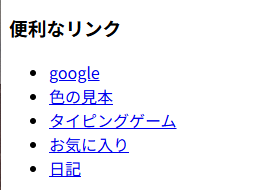
\includegraphics[width=0.4\textwidth]{../../asset/image/textbook-img193x.png}
  \caption{便利なリンク}
  \label{fig:1.4.24}
\end{figure}

\noindent%
googleのページに移動しましたか？
では、前のページに戻りましょう。
戻るには、ブラウザの左上にある戻るボタンをクリックします。
次に、\ul{タイピングゲーム}をクリックしてみてください。
実は、まだハイパーリンクの命令が記述されていませんので、ページは移動しません。
ここでは、ハイパーリンクが機能するように、命令を書いていきます。

まずは、タイピングページの住所（URL：uniform resource locator と呼ばれます）を調べましょう。
ブラウザで、タイピングゲームのページを開いてください。
開いたら、赤線の引いてある住所にあたる部分（URL）をクリックします。
その後で、右クリックして、メニューの「\textbf{すべてを選択(A)}」をクリックします。

\begin{figure}[htbp]
  \centering
  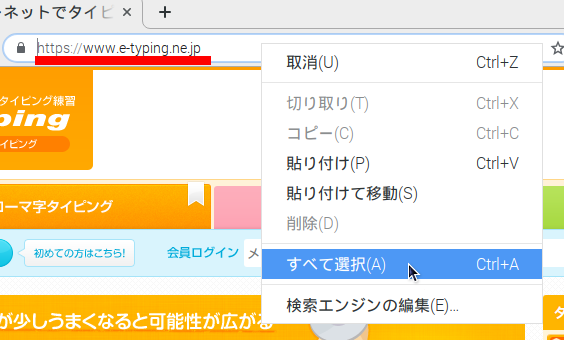
\includegraphics[width=0.45\textwidth]{../../asset/image/textbook-img196.png}
  \caption{URLを選択}
  \label{fig:1.4.25}
\end{figure}

\noindent%
すると、住所の情報がすべて選択されて、青く表示されますので、さらにそこで右クリックして、
メニューの「\textbf{コピー(C)}」をクリックします。
これで住所にあたる部分（URL）がコピーされました。
\clearpage

\begin{figure}[htbp]
  \centering
  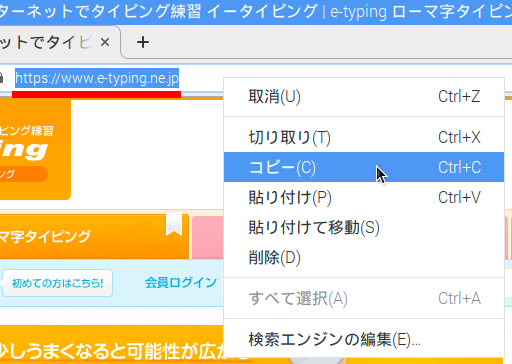
\includegraphics[width=0.4\textwidth]{../../asset/image/textbook-img197.png}
  \caption{URLのコピー}
  \label{fig:1.4.26}
\end{figure}

次に、テキストエディタで中身を見てみましょう。
\bigskip

\begin{lstlisting}[caption=ハイパーリンク（編集前）,label=pwdtest,firstnumber=1]
  <!-- 例題 1-27 自分の好きなウェブサイトを紹介しよう -->
  <h3>便利なリンク</h3>
    <!-- 番号なしのリスト(番号の代わりに・から始まる) -->
    <ul>
      <!-- リストの中身はliタグで作るよ
      リストの中身にはaタグを使っている 
      hrefでウェブサイトの場所を指定するよ -->
      <li><a href="https://google.com/">google</a></li>
      <li><a href="https://www.colordic.org/m/">色の見本</a></li>
      <#red#<li><a href="">タイピングゲーム</a></li>#>
    </ul>
\end{lstlisting} 

\noindent%
赤字で示したタイピングゲームを見てください。
上の行と違って、\texttt{href=""}の中身が\ruby{空}{から}になっていることが分かります。
ハイパーリンクを作るためには、aタグ\texttt{<a href="">}～\texttt{</a>}を使用します。
\vspace{.5cm}

\texttt{<a href="ホームページの住所">表示するリンク名</a>}
\vspace{.5cm}

\noindent%
上のようにaタグのhref属性にホームページの住所（URL）を書いて、
ホームページに表示される文字列「表示するリンク名」を指定すると、
ハイパーリンクが作成されます。

では、\ul{タイピングゲーム}をハイパーリンクとして機能させるために、
href属性に、先ほどコピーした住所の情報をペーストしてみましょう。
\texttt{href=""}のダブルクオーテーションの中をクリックした後で、
右クリックしてメニューの「\textbf{\ruby{貼}{は}り付け(P)}」をクリックします。
\vspace{0.5cm}

\begin{lstlisting}[caption=ハイパーリンク（編集後）,label=pwdtest,firstnumber=1]
      <li><a href="https://google.com/">google</a></li>
      <li><a href="https://www.colordic.org/m/">色の見本</a></li>
      <li><a <#red#href="https://www.e-typing.ne.jp/"#>>タイピングゲーム</a></li>
\end{lstlisting} 

\noindent%
これで、タイピングゲームのページに移動するためのハイパーリンクが完成しました。
テキストエディタを保存して、ブラウザをリロードしてみましょう。
\ul{タイピングゲーム}をクリックして、タイピングゲームのホームページに移動することを
確認してください。



\begin{tcolorbox}[title=\useOmetoi,breakable]
  \begin{enumerate}
    \addex{自分の好きなホームページのハイパーリンクを2つ追加してみましょう。}
  \end{enumerate}
\end{tcolorbox}
\clearpage



%
% subsection 1.4.11
%
\subsection{教室の使うものリストを作ろう}

リスト（\ruby{箇条}{かじょう}書き）を作るには、ulタグ（順序なしリストタグ）を使います。
より詳しく説明すると、\texttt{<ul>}～\texttt{</ul>}の中に、\ruby{箇条}{かじょう}書きにしたい項目を、
ランキングのときと同じようにliタグ\texttt{<li>}～\texttt{</li>}で指定します。
\vspace{0.5cm}

%
\begin{minipage}{0.58\linewidth}
  \begin{lstlisting}[caption=リストの例,label=pwdtest,firstnumber=1]
    <ul>
      <li>リスト項目1</li>
      <li>リスト項目2</li>
    </ul>	
  \end{lstlisting} 
  \end{minipage}
% \hfill
% 
% \vspace{20pt}
\begin{minipage}{0.36\linewidth}
  \centering
  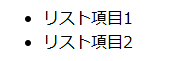
\includegraphics[width=0.5\linewidth]{../../asset/image/textfig_1001.png}
\end{minipage}
\bigskip

リストの中に、リストを入れることもできます。
テキストエディタで見てみましょう。
\vspace{0.5cm}

%
\begin{minipage}{0.58\linewidth}
  \begin{lstlisting}[caption=リスト（）,label=pwdtest,firstnumber=1]
    <!-- 例題 1-28 教室の持ち物リストを作ろう -->
    <h3>教室で使うものリスト</h3>
    <#red#<ul>#>
      <li>持ち帰るもの</li>
      <#blue#<ul>#>
        <li>ラズベリーパイ</li>
      <#blue#</ul>#>	
      <li>持ち帰らないもの</li>
      <#blue#<ul>#>
        <li>ディスプレイ</li>
      <#blue#</ul>#>
    <#red#</ul>#>
  \end{lstlisting} 
  \end{minipage}
\hfill
% 
% \vspace{20pt}
\begin{minipage}[t]{0.36\linewidth}
  \centering
  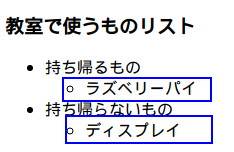
\includegraphics[width=0.7\linewidth]{../../asset/image/textbook-img204x.png}
\end{minipage}
\bigskip

\noindent%
外側のulタグの中に、さらに2つのulタグがあります。
このように、ulタグの中にulタグを使うと、リストの中でもリストが使えます。
\vspace{0.5cm}

% \begin{tcolorbox}[title=\useOmetoi,breakable]
%   \begin{enumerate}
%     \addex{「ラズベリーパイ」の下に、次の7個の項目をリストとして追加してみましょう（「電源ケーブル」、「HDMIケーブル」、「microSDカード」、「マウス」、「ヘッドセット」、「ウェブカメラ」、「GPIOエクステンダー」）。}
%   \end{enumerate}
% \end{tcolorbox}

\begin{minipage}{0.68\linewidth}
  \begin{tcolorbox}[title=\useOmetoi,breakable]
    \begin{enumerate}
      \addex{「ラズベリーパイ」の下に、次の7個の項目をリストとして追加してみましょう（「電源ケーブル」、「HDMIケーブル」、「microSDカード」、「マウス」、「ヘッドセット」、「ウェブカメラ」、「GPIOエクステンダー」）。}
    \end{enumerate}
  \end{tcolorbox}
\end{minipage}
\hfill
% 
\begin{minipage}{0.3\linewidth}
  \centering
  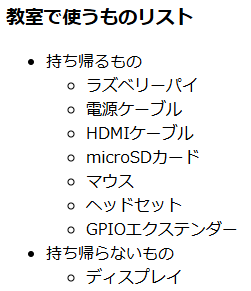
\includegraphics[width=0.9\linewidth]{../../asset/image/textfig_1002.png}
\end{minipage}

\clearpage


% では、練習として、「ラズベリーパイ」の下に、次の7個の項目をリストとして追加してみましょう
% （「電源ケーブル」、「HDMIケーブル」、「microSDカード」、「マウス」、「ヘッドセット」、
% 「ウェブカメラ」、「GPIOエクステンダー」）。
% \vspace{0.5cm}

% %
% \begin{minipage}{0.58\linewidth}
%   \begin{lstlisting}[caption=リスト（追加後）,label=pwdtest,firstnumber=1]
%     <!-- 例題 1-28 教室の持ち物リストを作ろう -->
%     <h3>教室で使うものリスト</h3>
%     <ul>
%       <li>持ち帰るもの</li>
%       <ul>
%         <li>ラズベリーパイ</li>
%         <#red#<li>電源ケーブル</li>
%         <li>HDMIケーブル</li>
%         <li>microSDカード</li>
%         <li>マウス</li>
%         <li>ヘッドセット</li>
%         <li>GPIOエクステンダー</li>#>
%       </ul>	
%       <li>持ち帰らないもの</li>
%       <ul>
%         <li>ディスプレイ</li>
%       </ul>
%     </ul>
%   \end{lstlisting} 
%   \end{minipage}
% \hfill
% % 
% % \vspace{20pt}
% \begin{minipage}[t]{0.36\linewidth}
%   \centering
%   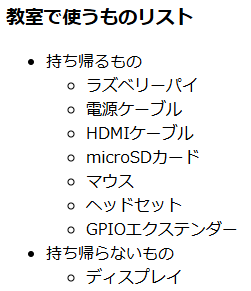
\includegraphics[width=0.7\linewidth]{../../asset/image/textfig_1002.png}
% \end{minipage}


\end{document}
